%----------------------------------------------------------------------------------------
%	PACKAGES AND OTHER DOCUMENT CONFIGURATIONS
%----------------------------------------------------------------------------------------


\documentclass[12pt,openright,oneside,final]{report}
\usepackage{generators/imports}
\makeglossaries

\renewcommand*{\acronymname}{List of Acronyms and Abbreviations}
\renewcommand{\glsnamefont}[1]{\textbf{#1}}

%Create acronyms here.
\newacronym{saas}{SaaS}{Software as a Service}
\newacronym{vcs}{VCS}{Version Control System}

%You can also do explanations.
\newglossaryentry{git}{name={Git},
    description={Git is a \gls{vcs} for tracking changes in computer files and coordinating work on those files among multiple people}}
\begin{document}
\begin{titlepage}

\newcommand{\HRule}{\rule{\linewidth}{0.5mm}} % Defines a new command for the horizontal lines, change thickness here

\center % Center everything on the page
 
%----------------------------------------------------------------------------------------
%	HEADING SECTIONS
%----------------------------------------------------------------------------------------

\textsc{\LARGE University of Bergen \\ Department of informatics}\\[1.5cm] % Name of your university/college

%----------------------------------------------------------------------------------------
%	TITLE SECTION
%----------------------------------------------------------------------------------------

\HRule \\[0.5cm]
\begin{Huge}
	\bfseries{Analysis of Word Embeddings: A Clustering and Topological Approach}\\[0.7cm] % Title of your document
\end{Huge}
\HRule \\[0.5cm]

%----------------------------------------------------------------------------------------
%	AUTHOR SECTION
%----------------------------------------------------------------------------------------

\large \emph{Author:} Jonas Folkvord Triki\\
\large \emph{Supervisor:} Nello Blaser\\[2cm]

%----------------------------------------------------------------------------------------
%   LOGO SECTION
% 	This will require the graphicx package
%	Change the line to comment if you only want the UiB Logo
%	Logo for other faculties here: http://kapd.h.uib.no/profilmanual/99LastNed/99a_lastned.html
%----------------------------------------------------------------------------------------

\centerline{
\includegraphics[scale=1.9]{figures/canvasWithFaculty}}
%\centerline{
\includegraphics[scale=0.15]{figures/canvas}}  %change for your faculty

%----------------------------------------------------------------------------------------
%	DATE SECTION
%----------------------------------------------------------------------------------------

{\large June, 2021}\\[3cm] % Date, change the \today to a set date if you want to be precise

%----------------------------------------------------------------------------------------
%	LOGO SECTION
%----------------------------------------------------------------------------------------

\vfill % Fill the rest of the page with whitespace

\end{titlepage}
 % This is the titlepage
\pagenumbering{roman}

\begin{abstract}
\noindent
Over the last few years, advances in natural language processing (NLP) have enabled us to learn more from textual data. To this end, word embedding models learn vectorized representations of words by training on big sets of texts (e.g. the entire Wikipedia corpus). Word2vec is a word embedding model which learns a single vector representation for each word it is trained on. However, by creating single vector representations for words, it becomes hard to separate between word meanings. Words with multiple meanings are called \textit{polysemous}, and determining the word meanings of a given word is a difficult problem in NLP. Traditionally, word embeddings from word2vec are analyzed using analogy and cluster analysis. In analogy analysis of word embeddings, it is common to show relationships between words, i.e that the relationship between \textit{king} and \textit{man} is same as that between \textit{queen} and \textit{woman}. Moreover, in cluster analysis of word embeddings, it is commonly shown that similar words cluster together, such as colours, names and countries. Additionally, recent developments in the field of topological data analysis (TDA) introduces a topological measure of polysemy, which attempts to identify polysemous words from their word embeddings. The goal of this thesis is to show how word embeddings traditionally are analyzed using analogies and clustering algorithms, and additionally, to use methods such as topological polysemy to identify polysemous words, using various word embeddings. Our results show that we are effectively able to cluster word embeddings into groups of varying sizes. Results also revealed that the measure of topological polysemy was inconsistent across word embeddings, and our proposed supervised models attempt to overcome and improve on this work.
\end{abstract}

\renewcommand{\abstractname}{Acknowledgements}
\begin{abstract}
I would first and foremost like to thank my supervisor, Nello Blaser, for his outstanding guidance during the work of this thesis.

I would also like to thank my fellow graduate students, particularly Naphat, for the long lunch breaks and the helpful academic discussions.

Finally, I would like to thank my friends and family for all their love and support.

\textbf{TODO}: Add to the acknowledgements.

\vspace{1cm}
\hspace*{\fill}\texttt{Jonas Folkvord Triki}\\ 
\hspace*{\fill} 01 June, 2021
\end{abstract}
\newpage
{\tableofcontents \let\cleardoublepage\clearpage \listoffigures \let\cleardoublepage\clearpage \listoftables \let\cleardoublepage\clearpage \lstlistoflistings}
\setcounter{secnumdepth}{4}
\setcounter{tocdepth}{4}
\pagenumbering{arabic}
\setcounter{page}{1}
\setlength{\parskip}{0.5cm plus4mm minus3mm}  

\chapter{Introduction}
\label{chap:introduction}
Natural language processing (NLP) is a field of study which focuses on the interactions between computers and the natural human language. In modern NLP applications, it is common to see the usage of vector embedding algorithms, such as the word2vec techniques introduced in \cite{mikolov2013a}. Word2vec learns vectorized representations of words (called word embeddings) by training on big text sets (e.g. whole Wikipedia). Word embeddings are created such that the semantics of a word is reflected by its word embedding. For example, the word \textit{solution} is similar to the word \textit{chemistry}, but is also related to words such as \textit{answer} or \textit{equation}. By inspecting the word embeddings of such words, we find that they are highly similar. Furthermore, we also see that the word \textit{solution} can have multiple meanings, depending on the context it is used in. We call such words \textit{polysemous}, and the task of determining polysemous words in NLP is a difficult problem. To measure and determine polysemous words from word embeddings, the measure of topological polysemy was introduced in \cite{jakubowski2020topology}. The topological polysemy method seeks to identify singular word embeddings, which the authors claim reflect polysemy.

Classically, word embeddings are analyzed using analogy and cluster analysis. In this thesis, we will first perform a similar analogy and cluster analysis, by using general methods from machine learning, and among these, clustering algorithms and dimensionality reduction methods. The goal is to find a richer description of word embeddings. In particular, we will first explain how we trained and evaluated our word2vec model, before proceeding onto clustering of word embeddings using clustering algorithms. We will validate the results from the cluster analysis using internal cluster validation methods and visualize our results using dimensionality reduction methods. After performing the cluster analysis on word embeddings, we will in this thesis investigate the method of topological polysemy by applying it to various word embedding models. Our goal is to recreate the results shown in \cite{jakubowski2020topology} for a general word embedding model, which further strengthens their proposed method and results. We will also look at another algorithm called Geometric Anomaly detection (GAD). GAD seeks to identify singular points in the data, similar to what the topological polysemy method does. Following, we will compare the results using topological polysemy and GAD to show their relation. Next, we look at the application of intrinsic dimension estimation (ID) methods on word embeddings and show the relationship between the estimated local ID of a word to the number of word meanings. We would like to, in particular, see if the estimated local ID of word embeddings can help us to predict the number of word meanings. Finally, we propose two supervised methods for predicting polysemous words, using results from topological polysemy, GAD and ID estimation methods.

This thesis is structured as follows. In \cref{chap:background} we give the technical and theoretical background required for this thesis. Following, in \cref{chap:analysis-of-word-embeddings} we perform our analysis of word embeddings, explaining training and evaluation steps for our word2vec model, perform clustering of word embeddings, and finally, analyze methods for polysemous words prediction. In \cref{chap:summary-and-conclusion}, we summarize and conclude the thesis. Lastly, in \cref{chap:future-work} we look at ideas for future work related to the thesis.
\chapter{General machine learning methods}
In this master thesis, we will use several general machine learning methods in conjunction with each other. In this chapter we will introduce and explain these methods.

\section{Artificial Neural Networks (ANNs)}
In this section we will explain artificial neural networks (ANN). In particular, we will focus on multilayered neural networks (MLNN). We refer to \cite[Chapter 1]{Aggarwal18} and \cite{rong2016word2vec} when describing this section.

\begin{definition}
An artificial neuron (or unit) is a function which receives one or more inputs and a bias, and then sums them to produce an output, as illustrated in \cref{fig:artificial_neuron}; $\left\{ x_1, \ldots, x_K \right\}$ are the input values, $b$ is the bias, $\left\{ w_1, \ldots, w_K \right\}$ are the weights and $y$ is a scalar output. We denote $f$ as the activation function.
\end{definition}

\begin{figure}[H]
    \centering
    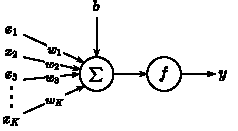
\includegraphics[width=8cm]{thesis/figures/artificial-neuron_cropped.pdf}
    \caption{An artificial neuron taking in a $K$-dimensional input $x$ and bias $b$ to produce some output $y$.}
    \label{fig:artificial_neuron}
\end{figure}

To produce the output of a single unit, we do the following
\begin{align}
    y = f(u)
\end{align}
where $u$ is the input of the neuron. $u$ is defined as
\begin{align}
    u = b + \sumlim{i=1}{K} w_i x_i
\end{align}
which is the weighted sum of the input values $\left\{ x_1, \ldots, x_K \right\}$ plus the bias term, with $\left\{ w_1, \ldots, w_K \right\}$ as weights.

The bias term acts as a intercept value to make the model more general and is usually set to +1. For some models (e.g. word2vec, introduced in \cref{sec:word2vec-as-an-ann}), one does not include the bias term for the units in the neural network, i.e., we leave $b$ to be zero.

The choice of activation function $f$ is typically a non-linear function. Artificial neural networks use different activation functions such as ReLU, sigmoid or tanh to learn non-linear relationships in the data. We will come back to this in \cref{sec:activation-functions-ann}.

\newcommand{\layer}[2]{\left\{ {#1}_{#2} \right\}}

\begin{definition}
\label{def:layer_ann}
A layer $\layer{z}{j} = \left\{ z_1, z_2, \ldots, z_K \right\}$ of an artificial neural network is a collection of artificial neurons (unit). More formally, the layer $\layer{z}{j}$ can be described using an $N \times K$-dimensional weight matrix $W$, a $N$-dimensional bias vector $b$ and an activation function $f$; see \cref{eqn:artificial_layer}.
\end{definition}

\begin{align}
    \layer{z}{j} = f \left( W \cdot x + b \right)
    \label{eqn:artificial_layer}
\end{align}
where $x$ is a $K$-dimensional input vector. In the following subsections, we will go over the different types of layers in the ANN, namely the input, hidden and output layers.

\subsection{Input layer}
\label{sec:ann-input-layer}
The first layer in the ANN is the input layer $\layer{x}{k} = \left\{ x_1, x_2, \ldots, x_K \right\}$. It is responsible for taking in input and passing it to the proceeding layer in the network. We illustrate the input layer in \cref{fig:input_layer_ann}.

\begin{figure}[H]
    \centering
    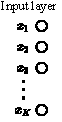
\includegraphics[height=7cm]{thesis/figures/artificial-neural-network-input-layer_cropped.pdf}
    \caption{Input layer in the ANN for a $K$-dimensional vector $x$.}
    \label{fig:input_layer_ann}
\end{figure}

More formally, we define the input layer in \cref{eqn:input_layer_ann} using \cref{def:layer_ann}. The layer does not perform any changes to the incoming data and acts as a way for feeding data into the neural network. For this reason, \cref{eqn:input_layer_ann} uses the identity matrix $I_K$ as the weight matrix $W_{\layer{x}{k}}$, no bias (i.e. bias equal to zero vector) the identity function $id(x)=x$ as the activation function.
\begin{align}
    \label{eqn:input_layer_ann}
    \layer{x}{k}
    &= f_{\layer{x}{k}}(W_{\layer{x}{k}} \cdot x) \\
    &= id(I_K \cdot x) \\
    &= I_K \cdot x \\
    &= x
\end{align}
With this in mind, we look at the layer the input layer is connected to, namely the hidden layer.

\subsection{Hidden layer}
The hidden layer is the second layer in the ANN $\layer{h}{i} = \left\{ h_1, h_2, \ldots, h_N \right\}$, and is most commonly connected to the input layer. It should be noted, however, that we might have multiple hidden layers in the ANN (making the neural network deeper), connecting them to each other. For illustration purposes, we will assume that we only have one hidden layer in our neural network. The hidden layer is illustrated in \cref{fig:hidden_layer_ann}. Here we observe that every unit in the input layer is connected to the units in the hidden layer, as illustrated the lines. This is what we call fully connected layers, meaning that every unit is connected to each other.

\begin{figure}[H]
    \centering
    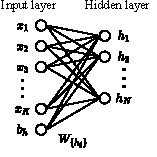
\includegraphics[height=7cm]{thesis/figures/artificial-neural-network-input-hidden-layer_cropped.pdf}
    \caption{Input to hidden layer in the ANN for a $K$-dimensional vector $x$, $N\times K$ dimensional weight matrix $\left\{ W_{h_i} \right\}$ and a $N$-dimensional hidden layer $h$.}
    \label{fig:hidden_layer_ann}
\end{figure}

We formalize the description of the hidden layer in \cref{eqn:hidden-layer-ann}
\begin{align}
    \label{eqn:hidden-layer-ann}
    \layer{h}{i} &= f_{\layer{h}{i}}(W_{\layer{h}{i}} \cdot \layer{x}{k} + b_h)
\end{align}
where $f_{\layer{h}{i}}$ is a user-specified activation function, $W_{\layer{h}{i}}$ is an $N \times K$-dimensional weight matrix and $b_h$ is an $N$-dimensional bias vector.

The hidden layer tries to learn a latent representation of the input data $x$. We will explain how the neural network learns the latent representation when introducing optimizers in \cref{sec:optimizers-ann}. Assuming that we have some $N$-dimensional latent representation of the data, we would like to connect it to the final layer in the neural network, namely the output layer.

\subsection{Output layer}
The last layer in the ANN is the output layer $\layer{y}{j} = \left\{ y_1, y_2, \ldots, y_M \right\}$ and is connected to the last hidden layer. Similar to the hidden layer, we connect each unit in the last hidden layer to each unit in the output layer, as illustrated in \cref{fig:mlnn-one-hidden}.

\begin{figure}[H]
    \centering
    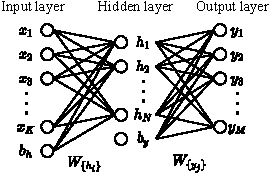
\includegraphics[width=9cm]{thesis/figures/artificial-neural-network_cropped.pdf}
    \caption{Multilayered neural network (MLNN) with one hidden layer.}
    \label{fig:mlnn-one-hidden}
\end{figure}

More formally, we define the output layer $\layer{y}{j}$ using a $M \times N$ weight matrix $W_{\layer{y}{j}}$, an $M$-dimensional bias vector $b_y$ and an activation function $f_{\layer{y}{j}}$, as seen in \cref{eqn:output-layer-ann}.

\begin{align}
    \label{eqn:output-layer-ann}
    \layer{y}{j} &= f_{\layer{y}{j}}(W_{\layer{y}{j}} \cdot \layer{h}{i} + b_y)
\end{align}

We have now covered the different layers in an MLNN, but have yet to cover the different choices of activation function $f$ in the neural network and how the MLNN learns.

\subsection{Activation functions}
\label{sec:activation-functions-ann}
The data which is fed into an ANN might contain complex patterns and have non-linear relationships. To deal with this problem, one applies an activation function to each layer before the result is sent to the proceeding layer. There are several choices of activation functions, and we will go over some of the most common ones.

The simplest type of activation is the identity function, as seen in \cref{eqn:identity-function}.
\begin{align}
    \label{eqn:identity-function}
    f(x) = x
\end{align}

The identity function is commonly used when we want to pass on the values from one layer to another without modifying the value itself, as we have already seen in \cref{sec:ann-input-layer}.

Other choices of activation functions include  sigmoid, tanh, Rectified Linear Unit (ReLU) and softmax, as illustrated in \cref{fig:activation-functions}.
\begin{align}
    \label{eqn:sigmoid-function}
    f(x) &= \frac{1}{1 + \exp{ \left( -x \right) }} \thickspace \text{(sigmoid function)} \\
    \label{eqn:tanh-function}
    f(x) &= \frac{\exp{ \left( 2x \right) } - 1}{\exp{ \left( 2x \right) } + 1} \thickspace \text{(tanh function)} \\
    \label{eqn:relu-function}
    f(x) &= \max{\left\{ x, 0 \right\}} \thickspace \text{(ReLU function)} \\
    \label{eqn:softmax-function}
    f(x_i) &= \frac{\exp \left( x_i \right)}{\sumlim{j=1}{K} \exp \left( x_j \right)} \thickspace \text{, $i \in \left\{ 1, \ldots, K \right\}$ (softmax function)}
\end{align}
where $K$ is the number of output values for the softmax layer.

\begin{figure}[H]
    \centering
    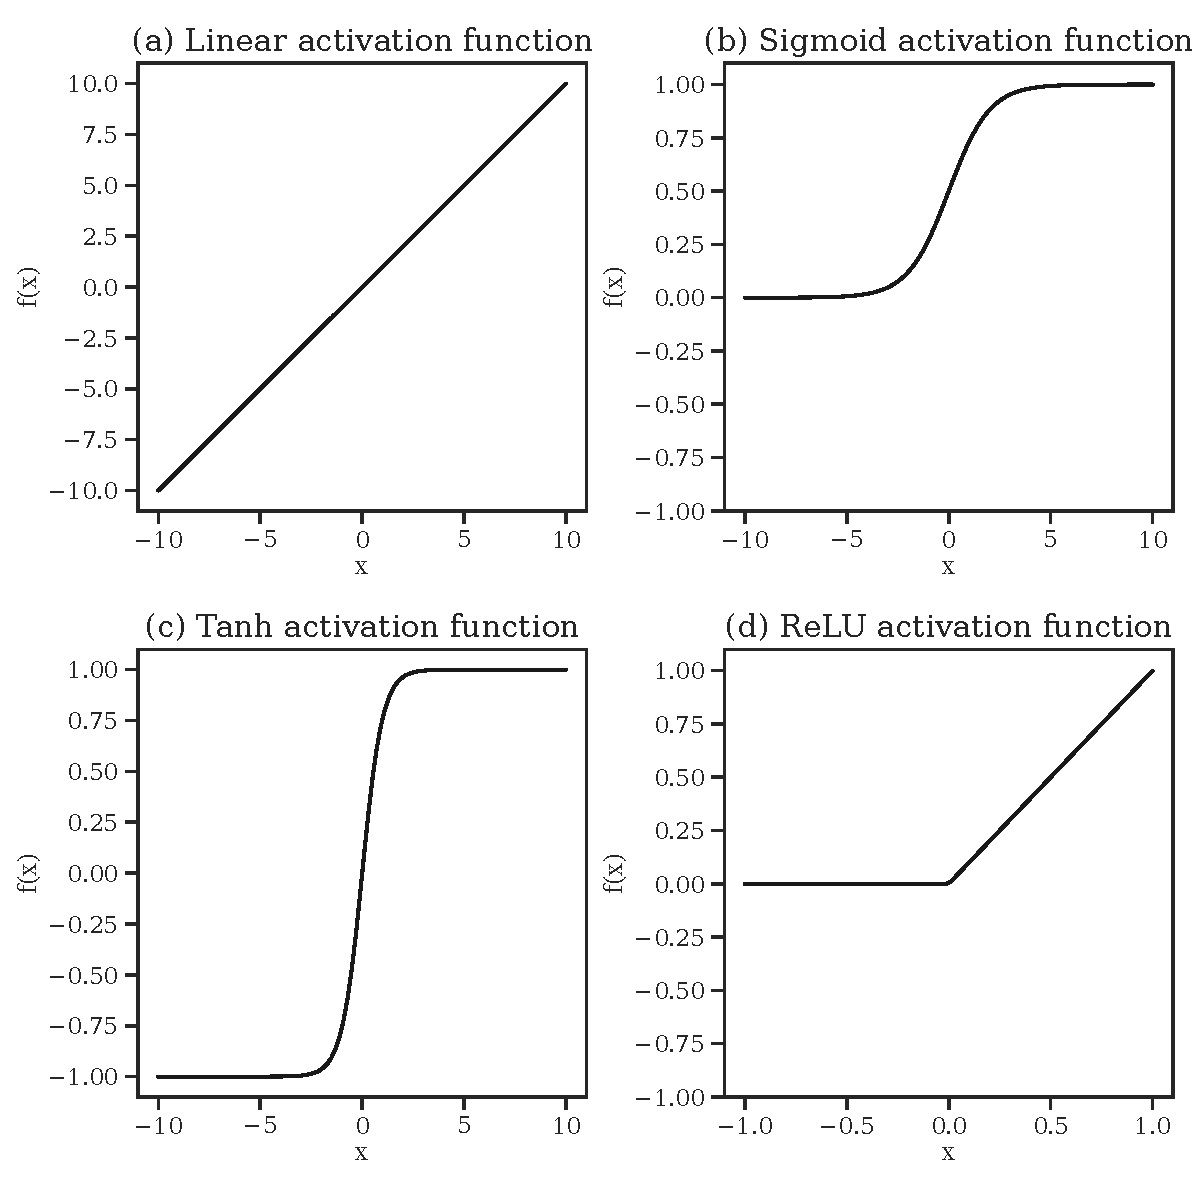
\includegraphics[width=0.7\textwidth]{thesis/figures/common-activation-functions.pdf}
    \caption{Various activation functions}
    \label{fig:activation-functions}
\end{figure}

The sigmoid and tanh activation functions were typically used in the early development of neural networks. The sigmoid activation function maps a value to a value in $(0, 1)$ and is particularly useful since it creates a probabilistic output. The tanh activation function has a similar shape to the sigmoid activation function, and maps values to values in $[-1, 1]$. In fact, the tanh and sigmoid activation functions are related, as illustrated in \cref{eqn:tanh-sigmoid-relation}.
\begin{align}
    \label{eqn:tanh-sigmoid-relation}
    \text{tanh}(x) = 2 \cdot \text{sigmoid}(2x) - 1
\end{align}

In recent years, the ReLU activation function has become more popular, partly due to its computational simplicity. In fact, both the sigmoid and tanh activation function suffers from vanishing gradients (i.e. gradients become zero, leading to very little learning) and ReLU is used as a substitute to overcome this problem. This does not mean, however, that the ReLU activation function can be used without problems, as it can "die out" since it is non-differentiable at 0. We will come back to this problem when introducing the gradient descent optimizer in \cref{sec:optimizers-ann}.

So far we have only discussed activation functions where we have a single output value. If we were to do a classification with $K$ outputs, one typically uses the softmax activation function. The softmax activation function is defined in \cref{eqn:softmax-function} and can be thought of the probabilities of the $K$ outputs.

\subsection{Loss functions}
\label{sec:loss-functions-ann}
So far we have seen how we can connect the different layers in an ANN. In short terms, we are given some input data, send it through some hidden layer and at last get the predicted output values from the output layer. We denote the predicted output values as $\hat{y}$. In this setting, we can assume that we have the true output labels, denoted as $y$. The loss function measures how much the predicted values $\hat{y}$ deviate from the true values $y$, and as such, the goal is to minimize this value. The output layer can have one or many outputs, and depending on the configuration of the network, the loss function changes as well. We separate the output types of an ANN into two categories, namely the regression and classification outputs.

In a regression type output, we usually predict some real-value quantity, such as height, weight or distance. For such problems, it is common to use the mean squared-error (MSE) loss. MSE is calculated as the mean of the squared differences between the predicted and true values, as seen in \cref{eqn:mse}.
\begin{align}
    \label{eqn:mse}
    MSE(\hat{y}, y) = \frac{1}{N} \sumlim{i=1}{N} {\left( y_i - \hat{y_i} \right)}^2
\end{align}
where $N$ is the length of $y$ and $\hat{y}$.

For classification type outputs, we want to classify whether or not some input data belongs to two (binary, e.g., on or off, blue or red) or more classes (categorical, e.g., different types of animals). In a binary classification type output, the sigmoid activation function in conjunction with the binary cross-entropy (BCE) loss function is used. The binary cross-entropy loss function is defined in \cref{eqn:binary-cross-entropy}.
\begin{align}
    \label{eqn:binary-cross-entropy}
    BCE(\hat{y}, y) = -\left( y \cdot \log{\left( \hat{y} \right)} + (1 - y) \cdot \log{\left( 1 - \hat{y} \right)} \right)
\end{align}
As opposed to the binary cross-entropy function, the categorical cross-entropy (CCE) function is used to compute the loss for multi-class classification output. It is common to see the usage of the softmax activation function being used at the output layer to create a multi-class probability distribution. Furthermore, we define the CCE loss function in \cref{eqn:categorical-cross-entropy} and observe that is is simply a generalization of the BCE loss function for multiple classes.
\begin{align}
    \label{eqn:categorical-cross-entropy}
    CCE(\hat{y}, y) = -\sumlim{c=1}{C} y_c \cdot \log{\left( \hat{y_c} \right)}
\end{align}
where $C$ is the number of classes in the multi-class classification output.

\subsection{Optimizers}
\label{sec:optimizers-ann}
In this subsection, we will discuss how an ANN is able to effectively make predictions from input data by learning its internal weights iteratively. In particular, we will look at the gradient descent algorithm and how ANNs exploit it to efficiently perform training.

So far, we have discussed what we call the forward pass (or phase). A forward pass is simply the journey of the input data to the output layers where we in each step compute the output values at each layer and local derivatives using the current set of weights. Once we are at the output layer, the forward pass is complete and the backward pass commences. Recall that the objective of the neural network is to minimize the loss function. To do so, we compute the derivative of the loss function with respect to the weights in the input layer, using the chain rule from calculus. The derivative of the loss function tells the neural network which direction it should move each weight in to minimize the loss (i.e. in the negative direction of the derivative).

To give an example of forward and backward passes in an ANN, consider the example in \cref{fig:neural-network-example-backprop}.
\begin{figure}[H]
    \centering
    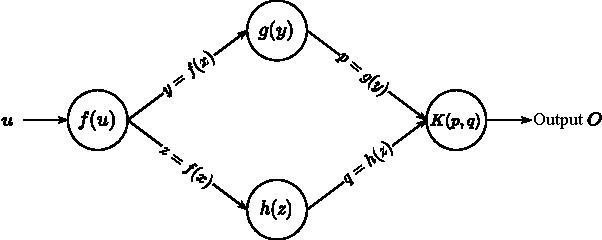
\includegraphics[width=12cm]{thesis/figures/artificial-neural-network-backprop-example_cropped.pdf}
    \caption{Neural network with one input node, one hidden layer with two nodes and a single output layer.}
    \label{fig:neural-network-example-backprop}
\end{figure}

In this example, we are given a network with one input node (neuron), a hidden layer with two nodes and a single output layer with one node. The input to the network is denoted as $u$ and is the product of the input data and the weights in the input layer. The activation functions of the network are denoted as $f$, $g$ and $h$. Moreover, the results of the activation functions are denoted as $y$, $z$, $p$, $q$, and the function $K$ combines the result of $p$ and $q$ resulting in the output value $O$. We assume that the weights of the hidden layer is applied to the previous layer's output values during $g$ and $h$ and the weights of the output layer is applied at $K$. The forward pass in this network is pretty straight forward; we start the input node, pass the data on to $g$ and $h$ and combine the results in the output layer. Now, for the backwards pass we first need to compute the loss at the output node using a loss function $L$. Furthermore, we compute the derivative of $L$ with respect to the input $u$. More formally, we need to compute
\begin{align}
    \parder{L}{u}
    &= \parder{L}{O} \cdot \parder{O}{u} \\
    &= \parder{L}{O} \cdot \left[
    \parder{O}{p} \cdot \parder{p}{u} +
    \parder{O}{q} \cdot \parder{q}{u}
    \right] \text{(chain rule)} \\
    &= \parder{L}{O} \cdot \left[
    \parder{O}{p} \cdot \parder{p}{y} \cdot \parder{y}{u} + 
    \parder{O}{q} \cdot \parder{q}{z} \cdot \parder{z}{u}
    \right] \text{(chain rule)} \\
    &= \parder{L}{O} \cdot \left[
    \undertext{\parder{K(p, q)}{p} \cdot g'(y) \cdot f'(u)}{Path on top} + 
    \undertext{\parder{K(p, q)}{q} \cdot h'(z) \cdot f'(u)}{Path on bottom}
    \right]
\end{align}

With this example in mind, we have illustrated how the derivatives are being calculated for a small neural network. There exists, effective and more general frameworks to derive the derivative of the loss with respect to the input values, but we will leave those details out and kindly refer the reader to \cite[Chapter 1.3]{Aggarwal18} for more details.

We have now gone over the forward and backward passes, which are the first two steps of the so called backpropagation algorithm. The remaining step of the algorithm is now to use the computed derivatives to update the weights of the ANN. To do this, we use the gradient descent (GD) algorithm. The main idea of gradient descent is to update the weights iteratively by moving them in the opposite direction of the gradient (i.e. the steepest descent), and by doing so, we will hopefully reach some local minimum leading better to fitting weights for the input-output data. In standard gradient descent, we perform its steps in the following manner
\begin{align}
    W \Leftarrow W - \alpha \cdot \parder{L}{W}
\end{align}
where $W = \left( w_1, w_2, \ldots, w_d \right)$ is the matrix consisting of the $d$ weights of an ANN. The learning rate $\alpha$ is a hyperparameter and determines how much learning we want to do in each step. The learning rate is usually set to a relatively low value, in the order of $10^{-2}$ to $10^{-5}$.

Even though gradient descent works great for small applications, once we scale the number of parameters (weights) in the ANN to the more extremes (e.g. in the order of millions), it becomes impractical to compute for the entire training data at once. Furthermore, we observe that a loss function $L$ usually can be written as a sum of the loss of the individual training data points (denoted $L_i$ for $i$th training point), as shown in \cref{eqn:loss-function-sum-individual}.
\begin{align}
    \label{eqn:loss-function-sum-individual}
    L = \sumlim{i=1}{n} L_i
\end{align}
Using the observation that we are able to write the loss function as the sum in \cref{eqn:loss-function-sum-individual}, we introduce the stochastic gradient descent (SGD) method. Instead of performing gradient descent on the whole input data, SGD instead performs gradient descent for each input data separately, as shown in \cref{eqn:sgd}. We call it stochastic, because a random sample of the training data is chosen for each iteration.
\begin{align}
    \label{eqn:sgd}
    W \Leftarrow W - \alpha \cdot \parder{L_i}{W}
\end{align}
where $n$ is the number of input data points and $L_i$ represents the loss the $i$th input. An advantage SGD has over GD, is that it runs a lot faster, at the expense of greater loss. Thankfully, there exists a variant of SGD which seeks to find a balance between speed and loss, namely the mini-batch stochastic gradient descent. In mini-batch stochastic gradient descent, one uses a batch $B=\enclc{j_1, \ldots, j_m}$ of input training data indices when computing the weight updating, as shown in \cref{eqn:mbsgd}.
\begin{align}
    \label{eqn:mbsgd}
    W \Leftarrow W - \alpha \cdot \sumlim{j \in B}{} \parder{L_j}{W}
\end{align}
Mini-batch stochastic gradient descent often finds the best trade-off between stability, speed and memory requirements. It should be noted, however, that the memory requirement increases with the use of mini-batches, due to the fact that we have to store bigger matrices in memory during training. One typically chooses batch sizes that are power of 2 (e.g. 32, 64, 128 or 256), since most modern hardware architectures are optimized for it.

In addition to the different variants of gradient descent, there exist a bunch of other variants which can solve issues such as getting stuck in local minimas or speeding up the training process. We will not go into detail on all these strategies here, but kindly refer the reader to \cite[Chapter 3.5]{Aggarwal18} for more details.

\section{Clustering techniques}
In a supervised machine learning setting, we usually are given some data $X$ and associated labels $y$. The supervised task is to train a model to predict the labels $y$ given data $X$. A classical example of a supervised machine learning task is to distinguish between dogs and cats, where $X$ is an image of the dogs and cats and the labels $y$ indicate whether or not the data $X$ represents a dog ($y=0$) or a cat ($y=1$). In an unsupervised setting, however, the labels $y$ might not be present. To predict the labels $y$, clustering techniques are usually applied.

Clustering is one of the most important techniques in unsupervised machine learning. Clustering algorithms divides some data $X$ into clusters (groups) such that the data in each cluster are similar in some sense. An example of this is clustering by distance (e.g. euclidean). If we cluster by distance, we want the distance between any two data points belonging to the same cluster to be small. This distance is also referred to as the intracluster distance. Unfortunately, it is not enough to only minimize the intracluster distance, we also have to ensure that distance between the clusters is as large as possible. To measure the distance the distance between two clusters we measure the distance between two data points belonging to different clusters. The distance between clusters is called intercluster distance. If a clustering algorithm is able to create clusters such that we have small intracluster distance and large intercluster distance, it indicates that the cluster algorithm is good for the data at hand. We note, however, that data can be very complex and it can be very hard to find good clusters.

We will now go over some common clustering algorithms, explain how they work and discuss their strengths/weaknesses. In each of the clustering algorithms, we can assume that we are given some data $X = \enclc{x_1, x_2, \ldots, x_n} \in \R^{n \times d}$.

\subsection{k-means clustering}
The k-means clustering method \cite[Section 9.1]{bishop2006} is an unsupervised machine learning algorithm used to identify clusters in data. The algorithm uses an iterative approach to search for $k$ clusters, where $k$ is a pre-determined number of clusters (i.e. hyperparameter). There exists several variants of this algorithm and we will discuss two of them in later subsections (\cref{sec:mini-batch-k-means-clustering} and \cref{sec:k-medoids-clustering}). We will now explain the standard (and naïve) variant of the algorithm, usually referred to as Lloyd's algorithm, and we base this section on \cite[Section 9.1]{bishop2006}.

The standard k-means clustering algorithm works as follows. The first step is to determine the initial cluster means, or centroids. Since we want the algorithm to output $k$ clusters, we have to decide $k$ initial centroids. The simplest way to do this is to select $k$ random data points to be the initial $k$ centroids. The next step is to calculate the euclidean distance between each data point to the cluster centroids. We do so because we want to determine which cluster each data point belong to. Furthermore, we assign each data point to its closest cluster centroid and compute the mean of each cluster. The third and final step is to move the cluster centroid to the newly computed mean of each cluster. The second and third step is then repeated until the desired clustering is achieved.

More formally, the goal of k-means clustering is to minimize the squared distance between the points in each cluster to its respective centroid. This is also referred to as the within-cluster sum of squares (WCSS). The objective is to find
\begin{align}
    \argmin_{C} \sumlim{i=1}{k} \sumlim{x \in C_i}{} \norm{x - \mu_i}^2
\end{align}
where $C = \enclc{C_1, C_2, \ldots, C_k}$ are the clusters of the data $X$, $k$ is the desired number of clusters and $\mu_i$ is the cluster centroid of cluster $C_i$.

The main advantage of k-means clustering is its simplicity, both in implementation and interpreting the results. The algorithm also scales well to larger data sets and there is only one hyperparameter to tune (number of clusters $k$). As for the disadvantages, the algorithm is rather sensitive to the initialization of centroids in the first step. If we were to select very bad initial centroids, the convergence time of the algorithm increases greatly and we might not even get good clusters. We also have to choose the number of clusters manually, which is a downside if we have no additional knowledge of the data beforehand. In addition to this, the algorithm (as with any distance-based clustering algorithm) suffers from the curse of dimensionality (\cref{fig:curse-of-dimensionality}), i.e., the fact that when the dimensionality increases it becomes more and more difficult to distinguish between data points (all points converge to the same distance).

\begin{figure}[H]
    \centering
    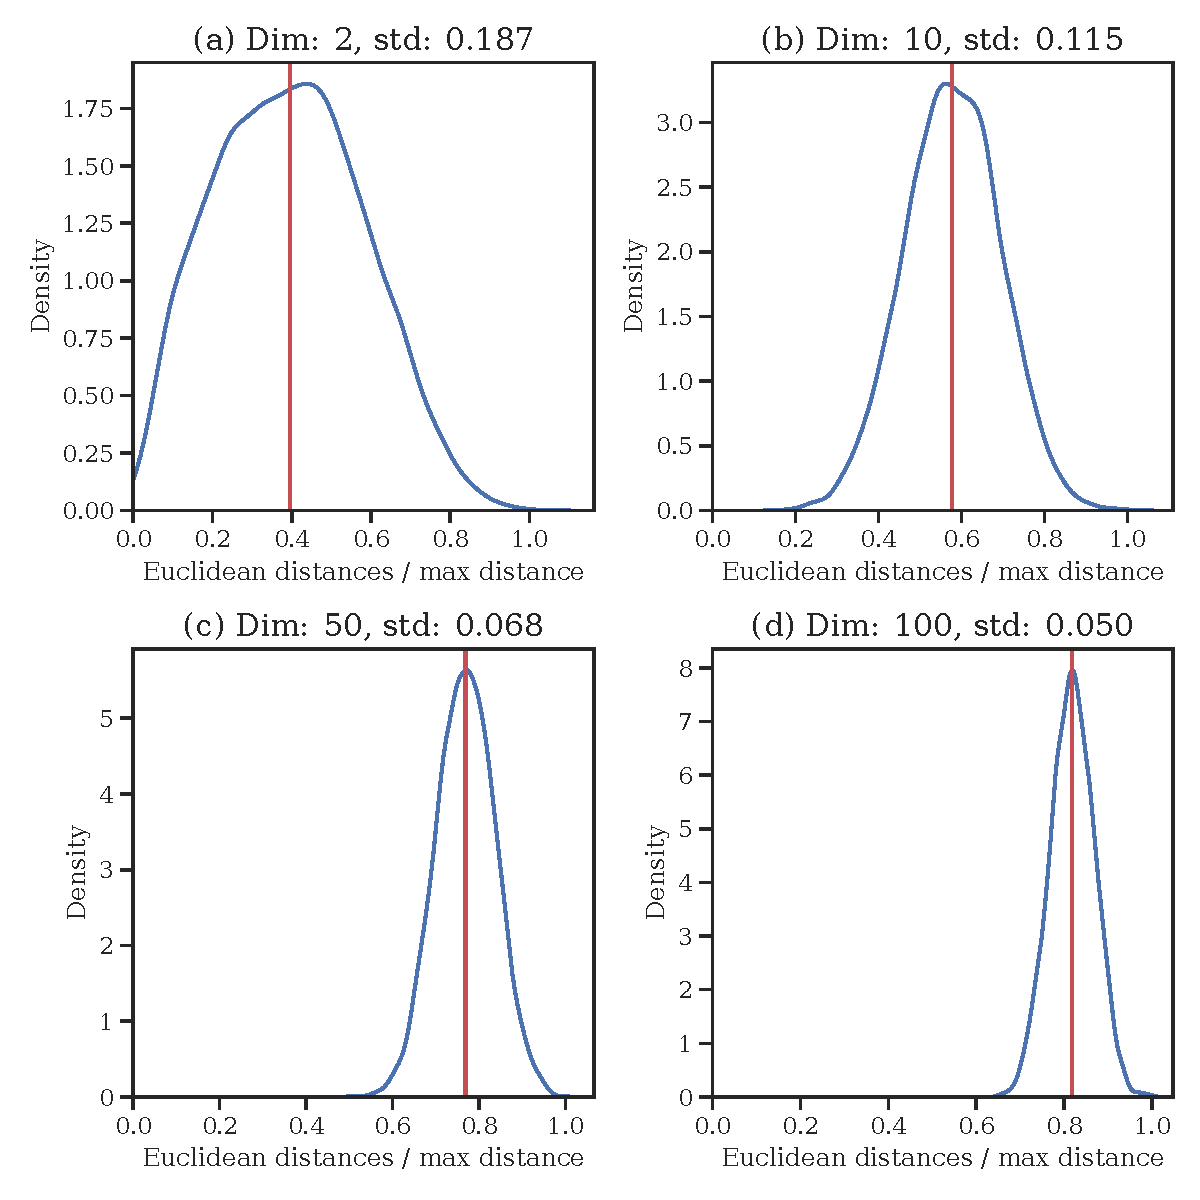
\includegraphics[width=0.7\textwidth]{thesis/figures/curse-of-dimensionality.pdf}
    \caption{Curse of dimensionality: the distance between points in higher dimensional spaces become the same as the dimensionality increases, and thus, it is harder to differentiate between points using distance metrics. The blue line represents the density of the pairwise euclidean distances (divided by max distance to normalize x-axis). The red line is the mean distance.}
    \label{fig:curse-of-dimensionality}
\end{figure}

\subsection{Mini-batch k-means clustering}
\label{sec:mini-batch-k-means-clustering}
The convergence time of K-means clustering depends on the number of data points $n$ and the desired number of clusters $k$. In order to reduce the computation time, mini-batch k-means clustering was introduced \cite{sculley2010}. The mini-batches are randomly sampled subsets of the training data for each training iteration (similar to the mini-batches in gradient descent). By using mini-batches, we drastically reduce the computational requirement required to converge to a local solution and, as noted by the authors in \cite{sculley2010}, the results of mini-batch k-means clustering tend to only be slightly worse than the standard algorithm.

The algorithm is very similar to the standard k-means clustering algorithm and comprises two major steps. In the first step, we initialize $k$ cluster centroids and sample $B=\enclc{b_1, b_2, \ldots, b_m} \subset X$ points at random from the data set $X$, where $m$ is the mini-batch size. In the second step, we update the cluster centroids by gradually moving the centroids. For each sample $b$ in the mini-batch, the centroids are updated by taking the average of $b$ and the previous points assigned to the centroid. By doing so, the centroid is moved with a decreasing rate over time. The first and the second step is repeated until convergence is met.

\textbf{TODO: Write cons/pros.}

\subsection{K-medoids clustering}
\label{sec:k-medoids-clustering}
K-medoids clustering was introduced as an alternative to the standard K-means clustering algorithm \cites{Kaufman1990}[p. 427 - 428]{bishop2006}. K-medoids clustering uses data points for its cluster centroids and works with any dissimilarity measures, making it more interpretable and robust to outliers than K-means clustering. A medoid of a cluster is a data point where the average dissimilarity between the medoid itself and all other data points in the same cluster is being minimized \cite{Kaufman1990}.

To solve the k-medoids problem efficiently, the Partitioning Around Medoids (PAM) algorithm is often used. Similar to the standard K-means clustering algorithm, PAM consists of two main stages called build and swap. In the build stage, we greedily select $k$ of the $n$ data points to be the initial cluster medoids, denoted $M = \enclc{m_1, m_2, \ldots, m_k} \subset X$. To select $M$ initially, we want to minimize the dissimilarity between the cluster medoids and associated points in the cluster. In other words, initially we set the first medoid $m_1$ to be the data point such that the dissimilarity between then medoid and all other data points is minimized. Then, for all proceeding medoids ($m_2, \ldots, m_k$), we look for medoids such that the dissimilarity between the additional medoid, the data points associated with the new medoid and all other medoids (and its associated data points) is minimized. This process is repeated until we have $k$ medoids. Following, the swap stage consists of iteratively swapping out the $k$ medoids with other data points from the data set, if it minimizes the overall dissimilarity. The algorithm terminates if by swapping the medoids with other data points we do not get lower dissimilarity.

Even though K-medoids clustering seems to be the superior choice over K-means clustering, it suffers from the fact it is more computationally heavy to compute and thus is not always feasible to run for large data sets.

\textbf{TODO: Write cons/pros.}

\subsection{Gaussian mixture models (GMMs)}
\label{sec:gmm-clustering}
Gaussian mixture models (GMMs) are probability distributions which consists of a mixture of multiple Gaussians \cite[Section 9.2]{bishop2006}. A Gaussian (also called normal) is a probability distribution which was several nice properties, such as mean as its mode and symmetry. In the context of cluster algorithms, GMMs can be used to cluster data points by using multivariate (i.e. of higher dimension) Gaussian distributions as cluster centroids. In particular, for each cluster centroid $c_i, 1 \leq i \leq k$, we define $\mu_i$ to be the cluster mean, $\Sigma_i$ to be the cluster covariances and $\pi_i$ to be the mixing coefficients. The cluster mean $\mu_i$ and covariances $\Sigma_i$ determines the localization and spread for each cluster, while the mixing coefficients $\pi_i$ determine how much we emphasize each cluster. In other words, by using Gaussian distributions, we get more freedom as to how the clusters are shaped and how much to prioritize them for each data point. To estimate the parameters $\theta = \enclc{\mu, \Sigma, \pi}$ of GMMs, the Expectation-Maximization (EM) algorithm is often used and is an iterative algorithm.

The EM algorithm starts off my initializing its parameters $\mu$, $\Sigma$ and $\pi$. There exists several methods for initializing the parameters and it is common to first run K-means clustering on the data in order to obtain a suitable starting point. By running K-means clustering first, the parameters are computed by using statistics from the result of K-means. Furthermore, the EM algorithm consists of two main stages, namely expectation and maximization. In the expectation stage compute the responsibilities for each data point in $X$ using the current set of parameters. With responsibilities, we mean how much each Gaussian is responsible for explaining a single data point in $X$. Next, in the maximization step, the responsibilities from the expectation step is used to update the parameters such that the likelihood $\text{P}(X | \theta)$ is maximized. The likelihood $\text{P}(X | \theta)$ tells us how good the set of parameters $\theta$ fits our data $X$. The exact derivation and update rules for each parameter is left out and we refer the reader to \cites[Section 9.4]{bishop2006} for more details. Once a suitable threshold is met with respect to $\text{P}(X | \theta)$, the algorithm terminates and we have converged to a set or parameters $\hat{\theta}$. Using the final parameters, $\hat{\theta}$ we predict which Gaussian (i.e. cluster) each data point in $X$ is associated with.

\textbf{TODO: Write cons/pros.}

\subsection{Hierarchical clustering}
Hierarchical clustering is a group of clustering algorithms which constructs clusters by recursively partitioning the data points of $X$ in top-down or bottom-up fashion \cite{Rokach2005}. These two methods are divided into what we call agglomerative- and divisive hierarchical clustering. Using agglomerative hierarchical clustering, each data point in $X$ starts off in their own cluster and are successively merged until all points are merged into a single cluster. In contrast to the agglomerative method, divisive hierarchical clustering starts off with all data points in $X$ in a single cluster. Then, the single cluster is divided into smaller clusters, until each point is in its own cluster. The output of an hierarchical clustering algorithm is a dendrogram, which represents the nested clustering structure. An example of a dendrogram is illustrated in \cref{fig:dendrogram-example}.
\begin{figure}[H]
    \centering
    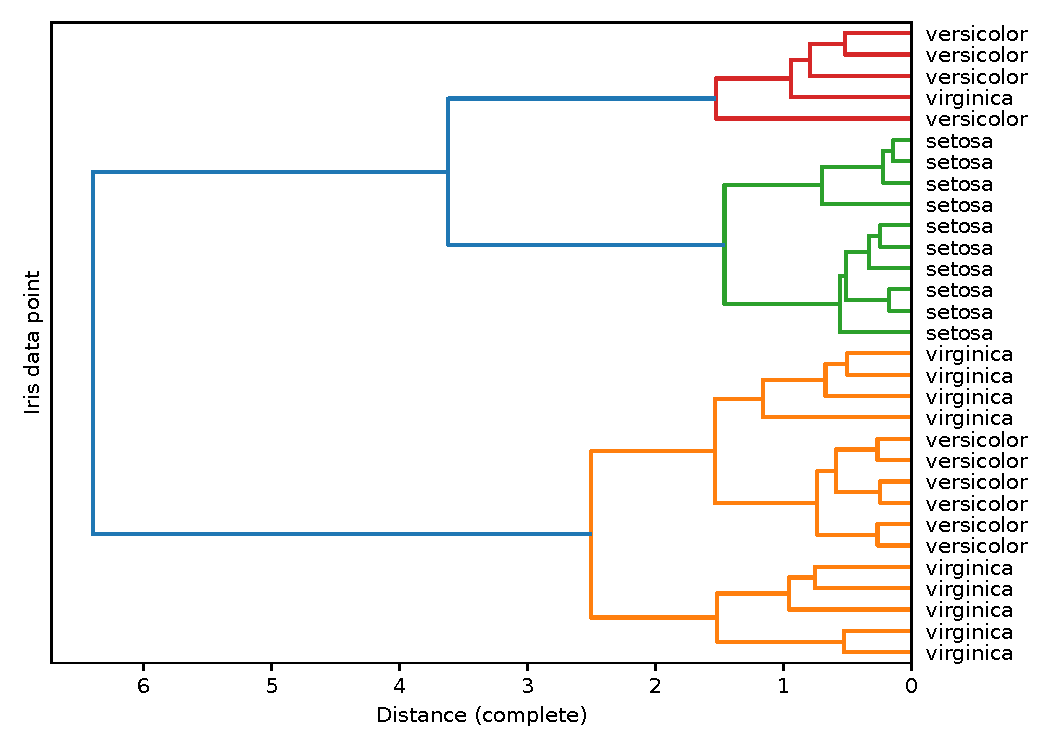
\includegraphics[width=0.9\textwidth]{thesis/figures/dendrogram-example.pdf}
    \caption{Example of a dendrogram plot using the Iris data set \cite{Fisher1936}.}
    \label{fig:dendrogram-example}
\end{figure}

To merge or divide clusters, we use some similarity measure in order to either merge similar data points (agglomerative) or divide dissimilar data points (divisive). Exactly which data points we choose to merge or divide depends on which criterion we want to optimize. There exist several different criterions one may choose to perform hierarchical clustering. Below we will list some of the most common ones and very briefly discuss the pros/cons for each criterion.
\begin{itemize}
    \item \textbf{Single-linkage clustering} --- combines two clusters that contain the closest pair (i.e. largest similarity) of elements that do not yet belong to the same cluster as each other.
    \begin{itemize}
        \item Single-linkage clustering tends to produce clusters of long chains, which can lead to the clustering of data points which in reality are far apart from each other.
        \item Single-linkage clustering is fast to use for big data sets and is able to create clusters of different shapes and sizes.
        \item Single-linkage clustering is sensible to noise.
    \end{itemize}
    \item \textbf{Complete-linkage clustering}  --- combines two clusters that contain the furthest pair (i.e. smallest similarity) of elements that do not yet belong to the same cluster as each other.
    \begin{itemize}
        \item Complete-linkage clustering is biased towards spherical clusters.
        \item Complete-linkage clustering works well on data with noise.
        \item Complete-linkage clustering tends to split large clusters.
    \end{itemize}
    \item \textbf{Average-linkage clustering} --- combines two clusters such that the average pairwise distance within the newly created cluster is minimum.
    \begin{itemize}
        \item Average-linkage clustering is biased towards spherical clusters.
        \item Average-linkage clustering works well on data with noise.
    \end{itemize}
    \item \textbf{Ward-linkage clustering} --- combines two clusters such that the variance of the newly created cluster is minimum \cite{Ward1963}.
    \begin{itemize}
        \item Ward-linkage clustering is biased towards spherical clusters.
        \item Ward-linkage clustering works well on data with noise.
    \end{itemize}
\end{itemize}

\textbf{TODO: Write cons/pros.}

\subsection{Spectral clustering}
Spectral clustering is a clustering algorithm which uses the eigenvalues of the affinity matrix (e.g. a similarity matrix using pairwise euclidean distances) of the data $X$ to reduce the dimensionality of the data, before applying some common clustering algorithm, such as K-means clustering \cite{Andrew2002}.

Imagine that we want to cluster the data into $k$ clusters. Spectral clustering starts off with the construction of the affinity matrix $A$. Typically, one uses some similarity measure to create pairwise distances between data points to create such an affinity matrix. Then, the graph Laplacian $L = D - A$ is computed, where $D$ is a diagonal matrix with $D_{ii} = \sumlim{j}{} A_{ij}$ and $A$ is the affinity matrix. The graph Laplacian $L$ is simply a matrix representation of a graph, and in our case, the similarities between data points in $X$. Next, the eigenvectors of $L$ is computed, and using these eigenvectors, we now have a lower-dimensional space of the original data $X$ (from $d$ dimensions to $k$). Lastly, we use a clustering algorithm, such as K-means clustering, on the eigenvectors of $L$ to get the final clustering.

\textbf{TODO: Write cons/pros.}

\subsection{HDBSCAN}
Clusters come in different shapes and sizes, and real-life data is rather noisy. DBSCAN is a density-based algorithm invented to cope with such problems \cite{Ester1996}. It, however, is only able to produce a "flat" clustering given some global threshold parameter. HDBSCAN is a generalization of DBSCAN and improves on it by creating a complete density-based clustering hierarchy \cite{Campello2013}, automatically extracting flat clusters. HDBSCAN is different from the other clustering algorithms we have seen so far, as it is able to create clustering without predetermining the number of clusters beforehand and can mark data points a noise. To fully understand the HDBSCAN algorithm, we will introduce its key concepts and then explain how the algorithm works in practice.

HDBSCAN is a density-based clustering algorithm and, for this reason, requires an inexpensive density estimation method to be efficient. Using k-nearest neighbours, the authors of HDBSCAN is able to estimate the density in an efficient manner. In particular, they define the \textbf{core distance} of a data point $x \in X$ to be the distance to the $\textit{minPts}$-nearest neighbour (including $x$), denoted $d_{core}(x)$. $\textit{minPts}$ is a hyperparameter and controls how conservative we want the clustering to be; the larger $\textit{minPts}$, the more points will be marked as "noise". To further spread apart data points that have low density, the \textbf{mutual reachability distance} metric (MRD) is defined, as seen in \cref{eqn:mutual_reachability_distance}.
\begin{align}
    d_{mreach}(x, y) = \max \enclc{ d_{core}(x), d_{core}(y), d(x, y) }
    \label{eqn:mutual_reachability_distance}
\end{align}
where $d(x, y)$ is the distance between data point $x$ and data point $y$ using the original distance metric. Under the MRD metric, data points in dense regions will not change their distances, but sparser data points will be pushed away such that the distance is at least their core distance to other points.

Next, given the MRD metric, we use it to find dense areas in the data. To find such areas, we create a minimal spanning tree (MST) where each node represents a data point $x \in X$ and edges connecting pairs of nodes is weighted by the MRD between the two nodes. By using an MST, we get a graph with the minimal set of edges between nodes such that the weight between the nodes is minimized. Also, by dropping one edge, we graph becomes disconnected, i.e., each pair of nodes is connected by exactly one edge. Using these two facts, we can create a clustering hierarchy in a single-linkage clustering manner. First, the weights of the edges of the MST is sorted in increasing order. Following, we iterate over the sorted edges of the MST and merge data points into clusters (note that each individual data point is its own cluster initially). Now, from the hierarchical clustering we are left with a dendrogram, as illustrated in \cref{fig:hdbscan-dendrogram-example}, but are left with a critical question; how should we define the cut in order to get a flat clustering?
\begin{figure}[H]
    \centering
    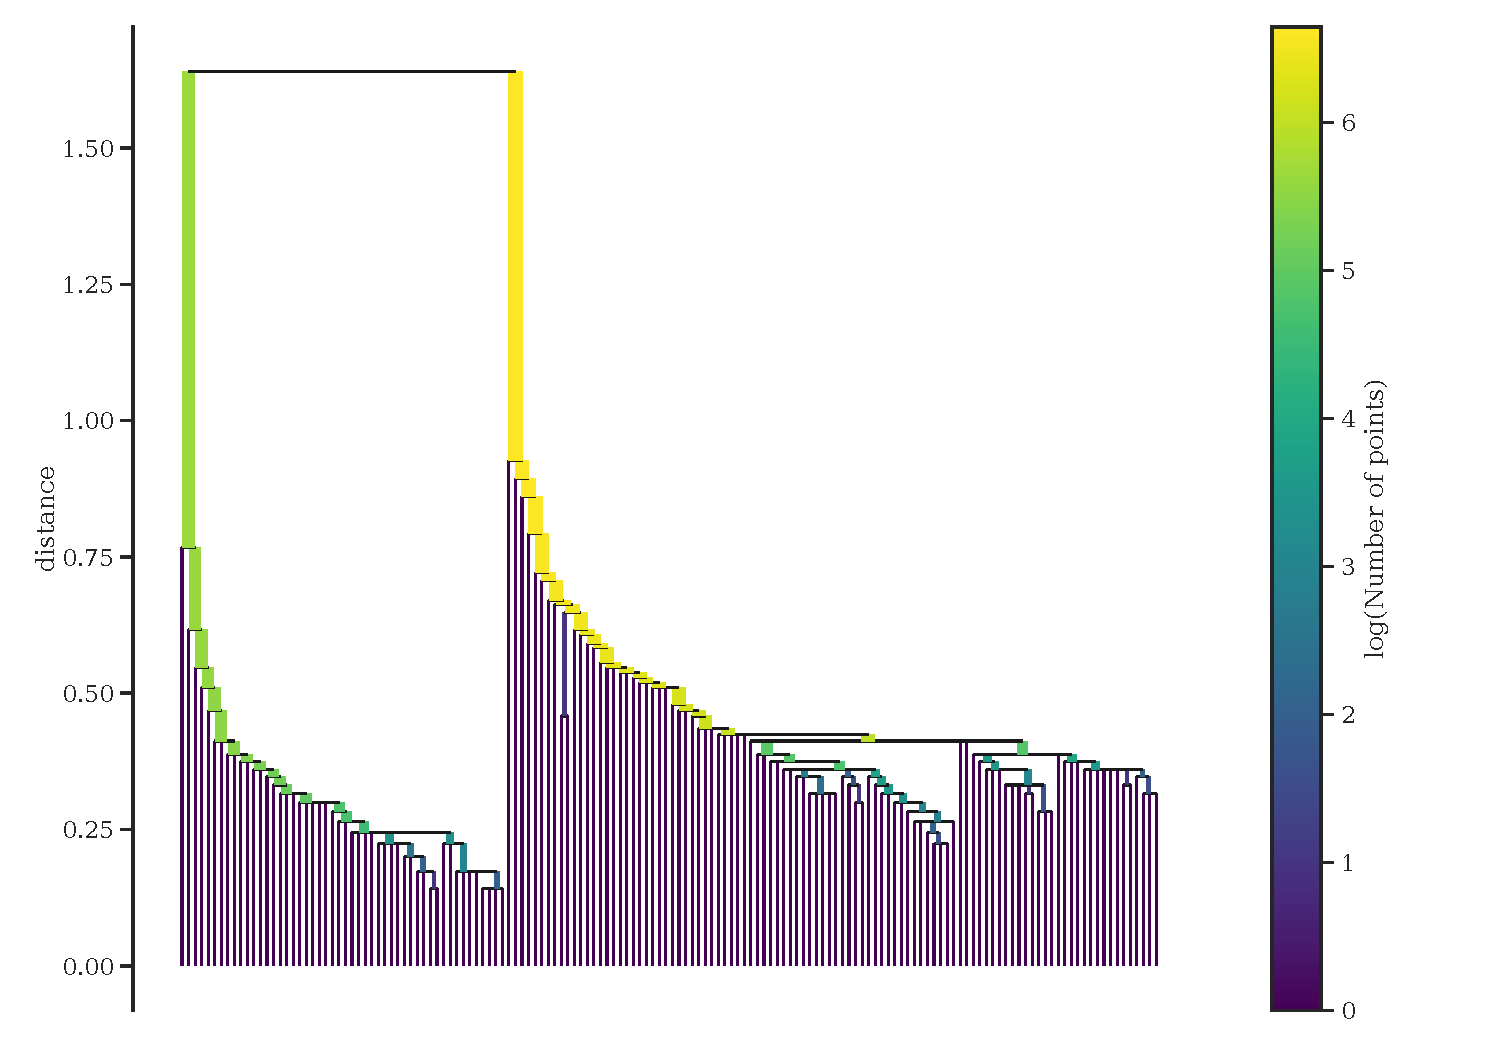
\includegraphics[width=10cm]{thesis/figures/hdbscan-single-linage-tree-example.pdf}
    \caption{Single-linkage dendrogram plot from HDBSCAN on the Iris data set \cite{Fisher1936}.}
    \label{fig:hdbscan-dendrogram-example}
\end{figure}

Dendrograms can be very difficult to interpret once a certain number of data points is reached. For this reason, the authors of HDBSCAN condense (or compact) the dendrogram from the hierarchical clustering such that a flat clustering can be obtained rather easily. First, the notion of \textbf{minimum cluster size} is defined and is a hyperparameter controlling the minimal cluster size at any time. Following, we walk down the dendrogram, starting from the root cluster, and at each split we check whether or not the new cluster created by the split has at least \textbf{minimum cluster size} data points in them. If the new cluster has at least \textbf{minimum cluster size} data points in them, we let that cluster be in the tree. If the new cluster has less than the \textbf{minimum cluster size}, then we let the parent cluster identify the new cluster and the node is removed from the tree. As we walk through the dendrogram in order to condense it, we also include at what distance clusters merge into the parent cluster, i.e., "fall out of clusters". An example of a condensed diagram is down in \cref{fig:hdbscan-condensed-dendrogram-example}.
\begin{figure}[H]
    \centering
    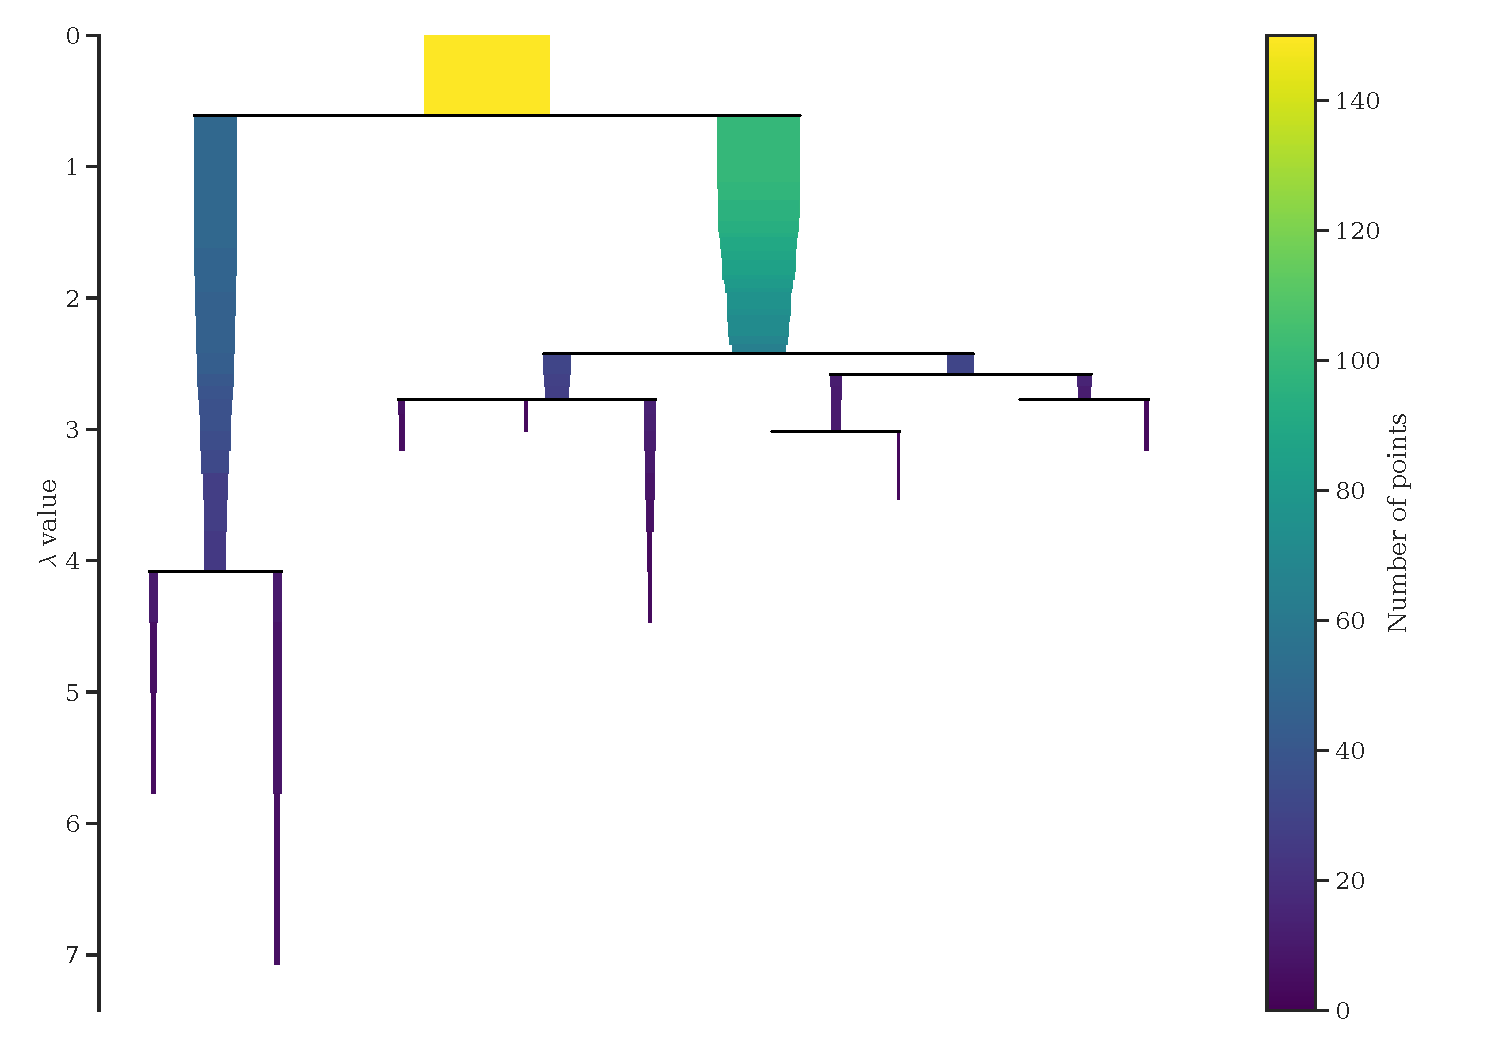
\includegraphics[width=10cm]{thesis/figures/hdbscan-condensed-tree-example.pdf}
    \caption{Condensed dendrogram plot from HDBSCAN on the Iris data set \cite{Fisher1936}.}
    \label{fig:hdbscan-condensed-dendrogram-example}
\end{figure}

Now, to define the flat cut in the condensed diagram, we select the clusters such that the largest total area of "ink" is maximized, under an additional constraint that we can not select clusters that are descendants of an already selected cluster. Any clusters which are not selected are marked as noise, as they are merely artifacts of the initial hierarchical clustering. The final clustering is then decided, as illustrated from the example in \cref{fig:hdbscan-condensed-dendrogram-final-cut-example}.
\begin{figure}[H]
    \centering
    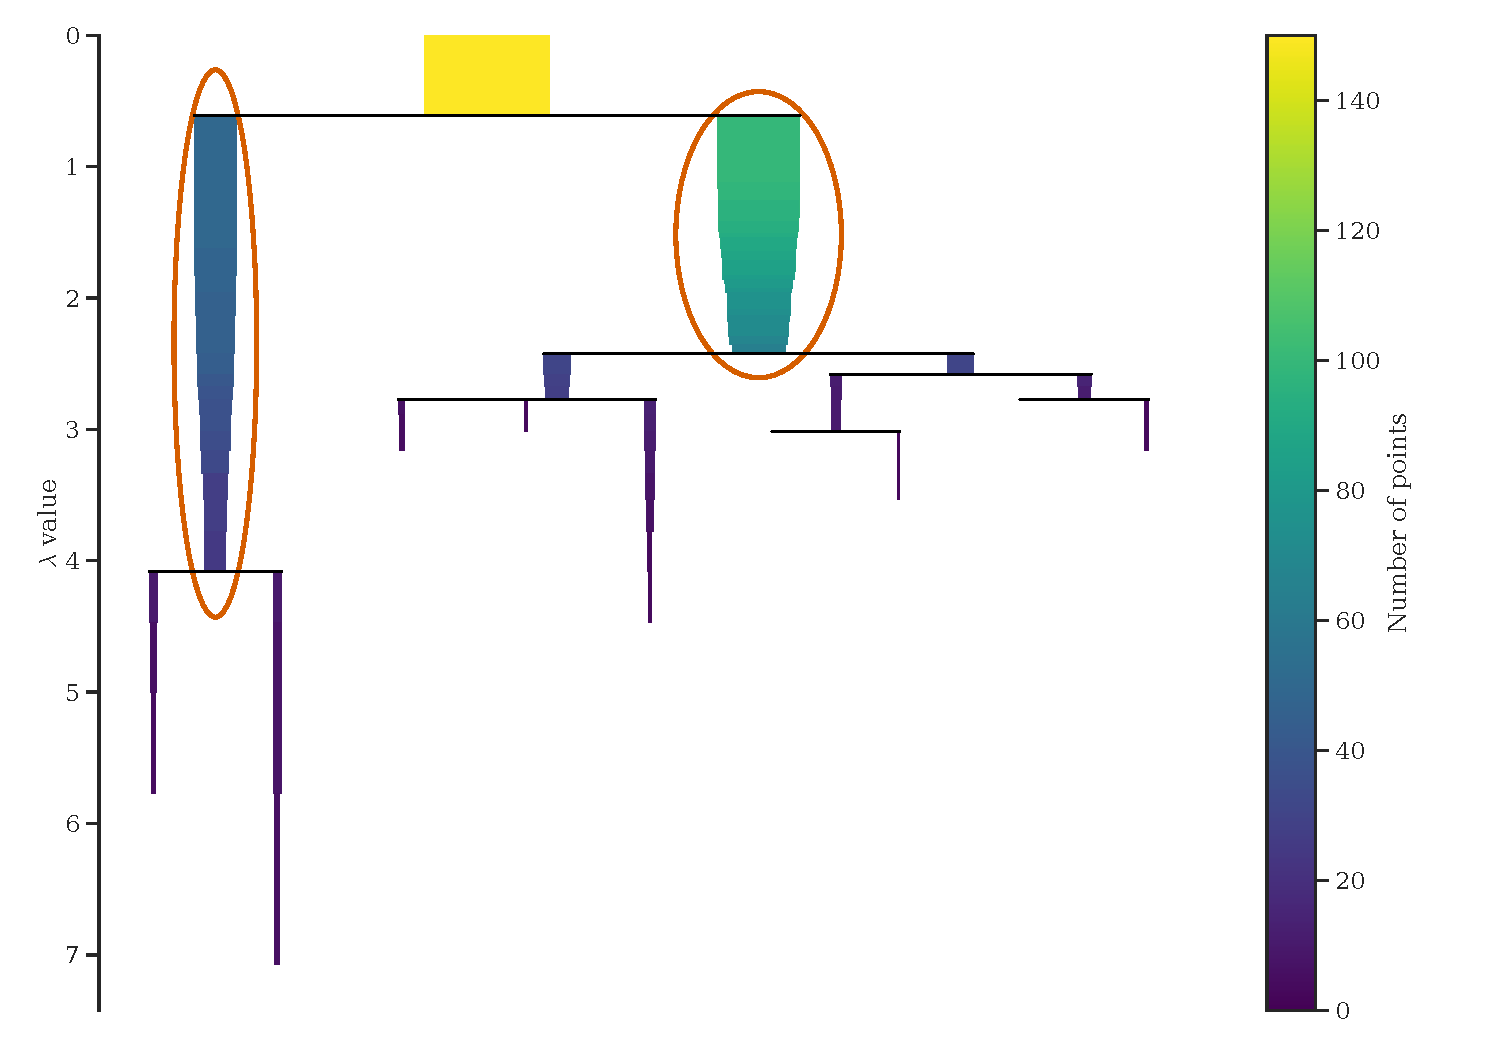
\includegraphics[width=10cm]{thesis/figures/hdbscan-condensed-tree-final-cut-example.pdf}
    \caption{Condensed dendrogram plot from HDBSCAN on the Iris data set \cite{Fisher1936}. The "final cut" is shown in the red circles. All data points below the circled clusters are considered noise.}
    \label{fig:hdbscan-condensed-dendrogram-final-cut-example}
\end{figure}

\textbf{TODO: Write cons/pros.}

\subsection{ToMATo}
Topological Mode Analysis Tool (ToMATo) \cite[2. ToMATo]{Oudot2015} is a clustering algorithm based on concepts from topological data analysis (TDA). In particular, ToMATo uses the concepts of persistence diagrams and prominence to perform clustering. We refer to \cite[2. ToMATo]{Oudot2015} when explaining the algorithm. The ToMATo clustering algorithm can be divided into three parts: density estimation and neighbour graph creation (1), mode-seeking (2) and merging (3).

First (1), any density estimation scheme is used in order to find dense areas in our data. A common choice is to use kernel density estimation with some kernel (e.g. gaussian). Let $\Tilde{f}(x_i)$ denote the estimated density of data point $x_i \in X, i = 1, 2, \ldots, n$. In addition to density estimation, a neighbourhood graph $G$ is computed in order to determine neighbours of data points. In the graph $G$, each vertex is a data point and edges represent neighbours. To compute $G$, it is common to use a $k$-nearest neighbour graph, where $k$ represents the number of neighbours.

Given the density estimator $\Tilde{f}$ and neighbourhood graph $G$, ToMATo uses mode-seeking (2) in order compute initial clusters. First, the vertices of $G$ are sorted by decreasing $\Tilde{f}$-value and iterated over. At each vertex $i$, compare the $\Tilde{f}$ values of vertex $i$ and its neighbours. If $\Tilde{f}(x_i)$ is greater than $\Tilde{f}$ of its neighbours, then vertex $i$ is denoted as a peak of $\Tilde{f}$. Otherwise, vertex $i$ is connected to the neighbour with the greatest  $\Tilde{f}$-value. By doing so, we create a spanning forest, where each spanning tree represent peaks of the underlying true density function. Given this spanning forest, the next step is to merge the trees to obtain a clustering.

The last step is the merging (3) of the spanning forest from (2). To do this, ToMATo iterates over the vertices of $G$ again (in the same order as in (2)) and a union-find data structure (denoted $\mathcal{U}$) is used to keep track of the merged spanning trees. The entries $e \in \mathcal{U}$ correspond to the union of spanning trees. The root of an entry $r(e)$, is the vertex in $e$ whose $\Tilde{f}$-value is the highest, i.e., a local peak of $\Tilde{f}$ in $G$. Now, iterating over the vertices of $G$, we check whether or not vertex $i$ is a peak of $\Tilde{f}$. If vertex $i$ is a peak of $\Tilde{f}$, i.e., root of some spanning tree $S$, a new entry $e$ is created in $\mathcal{U}$, in which $S$ is stored. The root of entry $e$ is set to the vertex itself, i.e., $r(e) = i$. If vertex $i$ is not a peak of $\Tilde{f}$, it means that it belongs to some existing entry $e_i \in \mathcal{U}$ and we look for potential merges of $e_i$ with other entries in $\mathcal{U}$. In particular, we iterate over neighbours $e \in \mathcal{E}$, $e \neq e_i$, of $i$ in $G$ and check whether $\min \enclc{ \Tilde{f}(x_{r(e)}), \Tilde{f}(x_{r(e_i)}) } < \Tilde{f}(x_i) + \tau$, where $\tau$ is the prominence threshold parameter. In other words, we check whether or not two entries have different $\Tilde{f}$-value and at least one of them has root with less than $\tau$ prominence. If this is true, $e$ and $e_i$ gets merged into a single entry in $\mathcal{U}$, i.e., $e \cup e_i$, and the entry with the lower root is merged into the one with the higher root.

Once the merging step is complete, we are left with a union-find structure $\mathcal{U}$. Every entry $e$ of $\mathcal{U}$ is connected to its parent entry $p(e)$ such that $\Tilde{f}(x_{p(e)}) > \Tilde{f}(x_e)$. In other words, by iteratively searching for the topmost parent, we can determine which cluster each entry (i.e. data point) is connected to. The ToMATo clustering algorithm can be seen as a combination of mode-seeking (from step (2)) and hierarchical clustering (from step (3)). As a result from the hierarchical structure, it is possible to visualize when entries in $\mathcal{U}$ gets merged into other entries, and thus, explain the lifespans of entries. More precisely, an entry in $\mathcal{U}$ is "born" when it is created in $\mathcal{U}$ and "dies" when it gets merged into another entry with higher root. Using persistence diagrams we can naturally explain the lifespans of entries and determine which entries live the longest (i.e. entries that never dies). The persistence diagram is also used to determine which value for $\tau$ we should use. Different values of $\tau$ results in different numbers of clusters. In practice, let $\tau = +\inf$ and use the persistence diagram of $\mathcal{U}$ to find a suitable threshold $\hat{\tau}$ such that the desired number of clusters is returned. Then, run ToMATo again using $\hat{\tau}$ as the threshold parameter to get the final clustering.

What is great about ToMATo is that it gives you a way to determine the numbers of clusters automatically (e.g. using some heuristic on the first persistence diagram to determine $\hat{\tau}$). In addition to this, ToMATo works with any metric, as long as a neighbourhood graph can be created using it (e.g. using euclidean distance or similar metrics).

\section{Cluster validation}
TODO: Introduce internal cluster validation

\subsection{Silhouette Coefficient}
TODO

\subsection{Davies-Bouldin index}
TODO

\subsection{DBCV}
TODO

\section{Dimensionality reduction techniques}
Working with data in high dimensions can be a difficult task at hand. Imagine that we have gathered some data, containing several features, and we would like to deepen our understanding of it. One approach we could do would be to visualize each feature by plotting them against each other, looking for bivariate relationships. Unfortunately, this is a rather cumbersome task and is hard to employ once a certain number of features is met (e.g. 10 features). Thankfully, dimensionality reduction techniques can help us to reduce the dimensionality of data into some lower dimension where relevant properties of the original data are preserved. A typical application of dimensionality reduction techniques is to lower the dimensionality to 2 or 3 such that one can visualize the data at ease. We will introduce two dimensionality reduction methods and explain how they work. In both subsections below, we assume that we are given some data $X \in \R^{n \times d}$ and that we want to reduce the dimensionality to some chosen hyperparameter $k$.

\subsection{Principal Component Analysis (PCA)}
Principal Component Analysis (PCA) is one of the most common dimensionality reduction techniques. PCA performs a linear mapping of the original data $X \in \R^{n \times d}$ to a (possibly) lower dimensional space $Y \in \R^{n \times k}$ ($k \leq d$) such that the variance is maximized in $Y$. One typically selects $k$ to a relatively low value, e.g., 2 or 3 if we would like to visualize the most varying part of the data or to a value such that a given variance threshold is met, e.g., explaining 90\% of the variance of the data.

The PCA algorithm consists of several steps and we will go through them briefly. First, the mean of $X$ is computed, denoted $\overline{X} = \frac{1}{n} \sumlim{i=1}{n} x_i$, and subtracted from $X$, i.e., $X' = X - \overline{X} = \enclc{x'_1, x'_2, \ldots, x'_n}$. Next, the covariance matrix of $X'$ is computed, denoted $C \in \R^{d \times d}$, and the corresponding eigenvectors and eigenvalues of $C$ are computed, denoted $C_\text{eig} = \enclc{c_1, c_2, \ldots, c_d}$. Furthermore, the eigenvectors $C_\text{eig}$ are sorted by its corresponding eigenvalues in a descending manner. By doing so, we get a set of ordered eigenvectors such that the first eigenvector corresponds with the largest value, the second eigenvector corresponds with the second largest value and so forth. We denote this set of ordered eigenvectors as $C'_\text{eig} = \enclc{c'_1, c'_2, \ldots, c'_d}$. We then pick the $k$ first eigenvectors of $C'_\text{eig}$ and project the data onto them, essentially performing a change of basis. In addition to this, the mean of $X$ is added to complete the reconstruction, as shown in \cref{eqn:pca-projection}.
\begin{align}
    \label{eqn:pca-projection}
    Y = X' \trans{\begin{pmatrix}
    c'_1 & c'_2 & \ldots & c'_k
    \end{pmatrix}} + \overline{X}
\end{align}
The newly created matrix $Y = \enclc{y_1, y_2, \ldots, y_n}$ represents the original data $X$ in (a possibly) lower dimension $k$, such that the variance in the vectors are maximized. The vectors $\enclc{y_1, y_2, \ldots, y_n}$ are also referred to as principal components (PC), where PC1 is $y_1$, PC2 is $y_2$ and so forth.

\textbf{TODO:} Add citation?

\subsection{Uniform Manifold Approximation and Projection (UMAP)}
Uniform Manifold Approximation and Projection (UMAP) is a dimensionality reduction algorithm based on, among other things, ideas from topological data analysis \cite{2018arXivUMAP}. In particular, UMAP uses a fuzzy version of simplicial complexes in order to create a weighted graph representing the topological structure of the data in higher dimension. To explain how the fuzzy version works, we will illustrate with the example from the "How UMAP Works" documentation page \cite{how-umap-works-2018}.

Imagine that we are given some data from a noisy sine, $X = \enclc{x_1, x_2, \ldots, x_n} \in \R^{n \times d}$, as illustrated in \cref{fig:how_umap_works_raw_data}.
\begin{figure}[H]
    \centering
    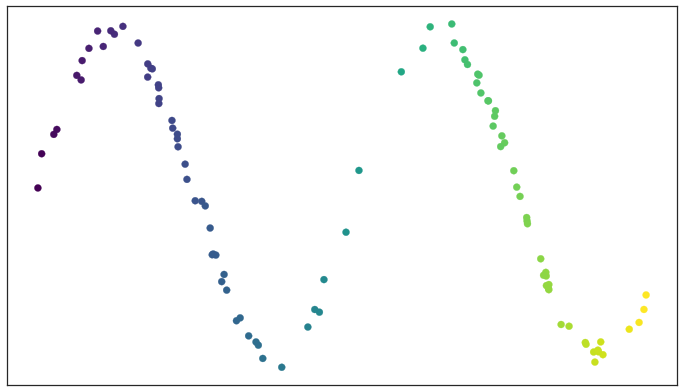
\includegraphics[width=10cm]{thesis/figures/how_umap_works_raw_data.png}
    \caption{Noisy sine wave (as illustrated by \cite{how-umap-works-2018}).}
    \label{fig:how_umap_works_raw_data}
\end{figure}

We would like to capture the topological structure of $X$, and we can do so by creating a simplicial complex built on $X$, illustrated in \cref{fig:how_umap_works_basic_graph}.
\begin{figure}[H]
    \centering
    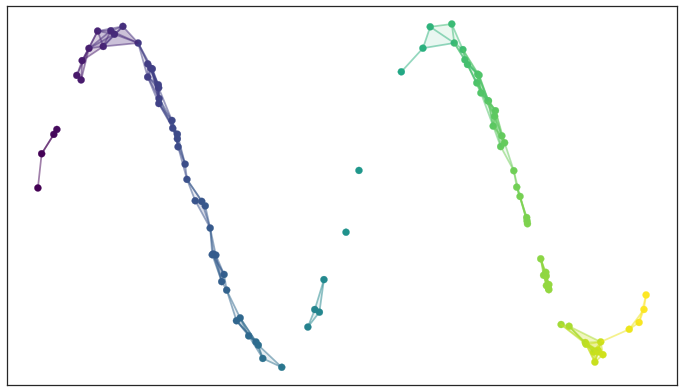
\includegraphics[width=10cm]{thesis/figures/how_umap_works_basic_graph.png}
    \caption{Simplicial complex built on a noisy sine wave (as illustrated by \cite{how-umap-works-2018}).}
    \label{fig:how_umap_works_basic_graph}
\end{figure}
We would like to capture the topological structure of all data points in $X$ and want a graph connecting all points. This, however is a problem, as there are some data points in \cref{fig:how_umap_works_basic_graph} which are disconnected from the simplicial complex, due to a small $\epsilon$ radius around each data point. In real word data, the data points are not uniformly distributed and selecting perfect $\epsilon$ to create a good simplicial complex is hard. The authors of UMAP overcome this problem by creating fuzzy open sets around each data point in order to create local connectivity in the graph, illustrated in \cref{fig:how_umap_works_umap_open_cover}.

\begin{figure}[H]
    \centering
    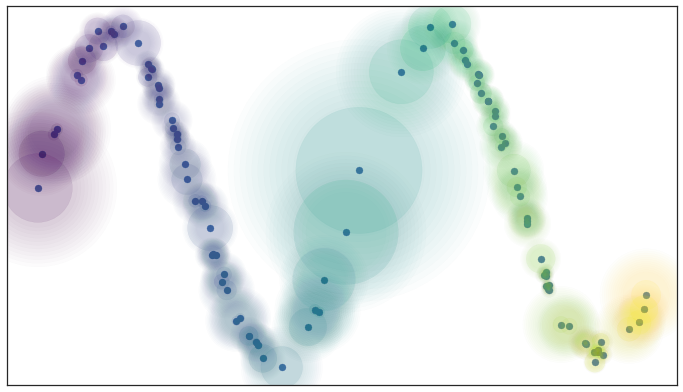
\includegraphics[width=10cm]{thesis/figures/how_umap_works_umap_open_cover.png}
    \caption{Fuzzy open sets around each data point of a noisy sine wave in order to create local connectivity (as illustrated by \cite{how-umap-works-2018}).}
    \label{fig:how_umap_works_umap_open_cover}
\end{figure}
To create the fuzzy open sets, the distance to the nearest neighbour of each data point is computed and the level of fuzziness decreases in terms of the distance beyond it, starting from 1 decreasing all the way to 0. If a data point has fuzziness level greater than zero, and edge is defined between the two data points, with fuzziness level as weight. We can also interpret the fuzziness level as the probability of the edge existing. We illustrate the connected graph in \cref{fig:how_umap_works_raw_graph}.

\begin{figure}[H]
    \centering
    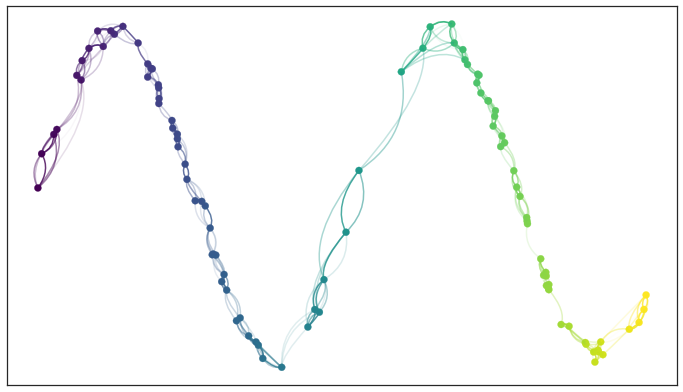
\includegraphics[width=10cm]{thesis/figures/how_umap_works_raw_graph.png}
    \caption{Connected graph where nodes are data points and edges between them are constructed given the fuzziness level between any two data point (as illustrated by \cite{how-umap-works-2018}).}
    \label{fig:how_umap_works_raw_graph}
\end{figure}
To finalize the connected graph from \cref{fig:how_umap_works_raw_graph}, the edges between any two data points gets converted into a single edge. We do this because we want the distance between two data points $a$ and $b$ to be the same; currently it depends locally on the distance to the nearest neighbour, as the fuzziness level decreases beyond it. To merge the edges between any two data points $a$ and $b$, the combined weight is computed by taking the union between them $w(a) + w(b) - w(a)w(b)$. This new combined weight is then used as weight of the single edge between $a$ and $b$. If we apply this process, unioning edges together, we end up with a fuzzy simplicial complex, illustrated in \cref{fig:how_umap_works_umap_graph}.

\begin{figure}[H]
    \centering
    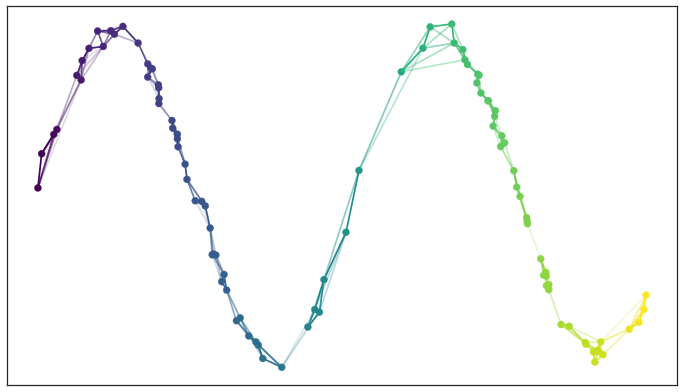
\includegraphics[width=10cm]{thesis/figures/how_umap_works_umap_graph.png}
    \caption{Fuzzy simplicial complex of some sine wave data (as illustrated by \cite{how-umap-works-2018}).}
    \label{fig:how_umap_works_umap_graph}
\end{figure}
Now, given the fuzzy simplicial complex of \cref{fig:how_umap_works_umap_graph}, we have a topological representation of $X$, capturing the topology of the manifold. We denote the set of all possible 1-simplices (i.e. edges) as $E$. The weight of a 1-simplex (i.e. edge) $e$ is computed using $w_h(e)$ in the high dimensional case. To get a good low dimensional representation of the high dimensional fuzzy simplicial complex, a low dimensional fuzzy simplicial complex is initialized and has weights denoted as $w_l(e)$ for edge $e$. To determine the weights $w_l(e)$, an iterative process is employed, where a loss function $L$ is optimized in a gradient descent fashion. Since we can interpret the weights of the 1-simplices of $E$ as probabilities of the edge existing (i.e. Bernoulli variables), the authors of UMAP uses cross-entropy as the loss function. More formally, the loss function $L$ is defined as
\begin{align}
    L = \sumlim{e \in E}{} \undertext{w_h(e) \log \enclp{\frac{w_h(e)}{w_l(e)}}}{Attractive force} + \undertext{(1 - w_h(e)) \log \enclp{\frac{1 - w_h(e)}{1 - w_l(e)}}}{Repulsive force}
    \label{eqn:umap-loss-function}
\end{align}

In the first term of \cref{eqn:umap-loss-function}, we have have an attractive force between the data points which $e$ spans, pulling them together; when $w_l(e)$ is large, the distance (i.e. weight) between any two data points becomes small. In the second term of \cref{eqn:umap-loss-function}, there is an opposite, repulsive force between the data points which $e$ spans, repelling them apart; when $w_h(e)$ is small (i.e. distance in high dimensional space), $w_l(e)$ will be small since we want to minimize the term. The process of pulling and repelling the weights makes the low dimensional representation of the data settle into a balanced state, such that it represents the high dimensional topological structure of the original data in a fairly accurate way. In practice, the UMAP algorithm uses a number of different tricks to optimize it, but we will not go into them here.
\chapter{Word embeddings}
In this chapter, we will discuss ways of representing text numerically, how we can create word embeddings and details around the word2vec technique from architectural choices to data preprocessing. At last, we will cover evaluation of word2vec models.

TODO: Change chapter introduction.

\section{Numerical representation of text}
Machine learning methods take in vectors (arrays of numbers) as input. When we want to work with text, we have to come up with some procedure for converting text into a vector, (i.e. vectorizing the text).
In this section, we will create some unique representation for words in a text, discuss one-hot encoding of words and the motivation behind creating word embeddings.

\subsection{Unique representation for each word}
\label{unique-representation-for-each-word}
A first strategy for vectorizing text could be to assign a unique number for each word in the text. We use the same order as the words appear in the text to assign a unique number. Furthermore, we define the number of unique words in the text to be the vocabulary size, denoted by $|V|$. We replace each word in the text with its respective number. Let us consider the following sentence
\begin{align}
    \text{the cat sat on the mat} \label{txt:num-rep-ex-sent-words}
\end{align}
\noindent
We convert the words into numbers based on the order they appear in the text, e.g., the $\mapsto$ 0, cat $\mapsto$ 1, sat $\mapsto$ 2, etc.
\begin{align}
    \text{0 1 2 3 0 4} \label{txt:num-rep-ex-sent}
\end{align}
We now have a numerical representation of the original sentence in $\ref{txt:num-rep-ex-sent-words}$ and may use it for machine learning modeling.

\noindent
There are some problems with this method, however.
\begin{itemize}
    \item The encoding of words into number is arbitrary (does not capture any relationship between words)
    \item Machine learning models might learn some natural ordering of the encodings, which can lead to bad results during inference. This is because the encoding of the words does not capture relationship between the words.
\end{itemize}

\noindent
In the next subsection, we will look at another method of encoding words, using one-hot encodings. We will also apply it to the example sentence in \ref{txt:num-rep-ex-sent-words}.

\subsection{One-hot encoded words}
One-hot encoding is a method for converting categorical data into numeric data. Essentially, we create a unique, sparse vector consisting of all zeros, except for the value at the index of the element of interest, which we set to one. For instance, if we have the words "north", "east", "south", "west", then their one-hot encodings could be
\begin{align}
    \text{north} \mapsto \begin{pmatrix}
    1\\
    0\\
    0\\
    0
    \end{pmatrix},
    \text{east} \mapsto \begin{pmatrix}
    0\\
    1\\
    0\\
    0
    \end{pmatrix},
    \text{south} \mapsto \begin{pmatrix}
    0\\
    0\\
    1\\
    0
    \end{pmatrix},
    \text{west} \mapsto \begin{pmatrix}
    0\\
    0\\
    0\\
    1
    \end{pmatrix}
\end{align}

\begin{definition}
Let $V = \left \{ w_1, w_2, ..., w_{|V|} \right \}$ denote the set of unique words in a text. Then, the one-hot encoding of a word, $e_{w_i}$, is defined as a $|V|$-dimensional vector of all zeros, except for the value at index $i$ which is one. \label{def:one-hot-encoding}
\end{definition}

\noindent
If we convert the numerical representation in \ref{txt:num-rep-ex-sent} using definition \ref{def:one-hot-encoding}, we get the following one-hot encoded vectors
\begin{align}
    \begin{pmatrix}
    1\\
    0\\
    0\\
    0\\
    0
    \end{pmatrix}
    \begin{pmatrix}
    0\\
    1\\
    0\\
    0\\
    0
    \end{pmatrix}
    \begin{pmatrix}
    0\\
    0\\
    1\\
    0\\
    0
    \end{pmatrix}
    \begin{pmatrix}
    0\\
    0\\
    0\\
    1\\
    0
    \end{pmatrix}
    \begin{pmatrix}
    1\\
    0\\
    0\\
    0\\
    0
    \end{pmatrix}
    \begin{pmatrix}
    0\\
    0\\
    0\\
    0\\
    1
    \end{pmatrix}
\end{align}
\noindent
We now have discarded the ordinal relationship of the numerical representation.

\noindent
There are some downsides with this approach as well, however.
\begin{itemize}
    \item As with the numerical representation in subsection \ref{unique-representation-for-each-word}, one-hot encoded vectors does not capture relationship between words.
    \item One-hot encoded vectors are sparse (meaning, most values are zero). Imagine if we had 1000 words in the vocabulary, then one would create a vector consisting of 99.9\% zeros. In practice, the vocabulary size is in the terms of $10^5$ to $10^7$ \cite{mikolov2013b}, e.g., by using one-hot encoded vector representations we are extremely inefficient in terms of space.
    \item One-hot encoded vectors are very high-dimensional (same as the number of words in the vocabulary, $|V|$).
\end{itemize}

\subsection{Word embeddings}
In contrast to the one-hot encoded vectors of words, word embeddings are low-dimensional dense vector representations. Word embeddings are typically learned from the data (e.g. texts) directly, whereas one-hot encoded vectors are statically defined. Due to the lower dimensionality of word embeddings, it packs more information about words into less space, thus being more efficient than one-hot encoded word vectors. Common choices for the dimensionality of word embeddings are ranging from 50 to 600 \cite{mikolov2013a}, depending on the amount of training data. We will take a look at a classic method of creating such word embeddings, called word2vec.

\section{Creating word embeddings (word2vec)}
Word2vec was first introduced by Mikolov et al. in 2013 \cite{mikolov2013a}. It is a family of techniques for learning dense and efficient vector representations of words. In the same year, Mikolov et al. introduced another paper which included several extensions that improved both the quality of the word embeddings and the training speed \cite{mikolov2013b}. In this section, we will go over the details of the original word2vec paper and the introduced extensions in the follow-up paper.

\subsection{Architectures}
The authors of the word2vec paper introduced two new log-linear models for learning distributed representations of words that try to minimize computational complexity, namely the continuous bag-of-words model (CBOW) and the continuous Skip-gram model. Both models achieve high quality word embeddings \cite{mikolov2013a} and share some core idea as to how one might create good vector representations of words. In this subsection, we will go through both models.

\subsubsection{Continuous bag-of-words model}
The continuous bag-of-words model (CBOW) tries to predict a target word given some context words around it. Essentially, we select a target word $w_t$, where $t$ is the index of the current target word in our training data, and a number $C$ denoting the number of words to the left and to the right of $w_t$. $C$ is also called the window size. By combining the projected word context vectors, we predict the target word $w_t$. This model is illustrated in \figref{fig:cbow-model}.

\begin{figure}[ht]
    \centering
    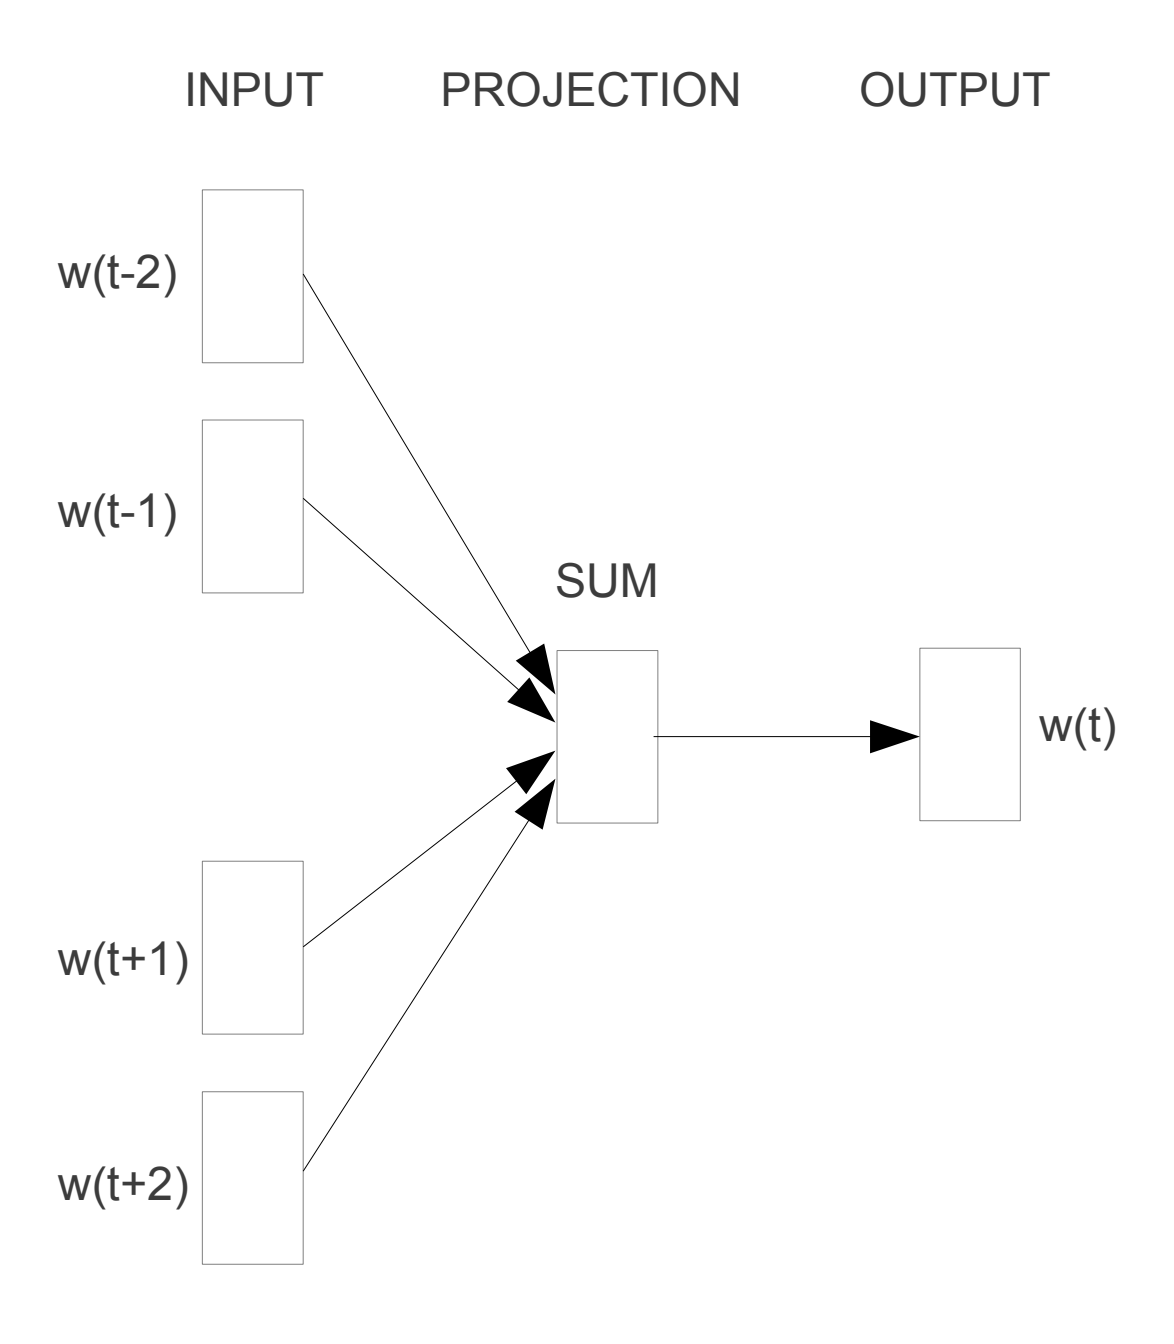
\includegraphics[width=8cm]{thesis/figures/cbow-mikolov-et-al-2013.png}
    \caption{CBOW architecture as illustrated by Mikolov et al. \cite{mikolov2013a}}
    \label{fig:cbow-model}
\end{figure}

\noindent
More formally, we are considering a sequence of $T$ training words $w_1, w_2, \ldots, w_T$. The words $w_t$ belong to some vocabulary $V$ consisting of $|V|$ unique words, $1 \leq t \leq T$. The models task is to maximize the average log probability of the word $w_t$ being sampled given the context words $w_{t-C}, \ldots, w_{t-1}, w_{t+1}, \ldots, w_{t+C}$. The objective of the CBOW model then becomes
\begin{align}
    \frac{1}{T} \sumlim{t=1}{T} \log p(w_t | w_{t-C}, \ldots, w_{t-1}, w_{t+1}, \ldots, w_{t+C})
    \label{eqn:cbow-objective-function}
\end{align}

\noindent
Through it is not clear from the original authors of word2vec \cite{mikolov2013a, mikolov2013b}, we typically use two weight matrices, $W$ and $W'$, when setting up the word2vec model \cite{rong2014word2vec}. The first weight matrix, $W$, is a $|V| \times D$ matrix, mapping the input word vectors (usually represented using one-hot encodings) to their internal embedding, where $|V|$ is the vocabulary size and $D$ is the number of dimensions in the hidden/projection layer. The second weight matrix, $W'$, is a $D \times |V|$ matrix mapping from the hidden/projection layer to the output prediction.

\subsubsection{Continuous Skip-gram model}
The continuous Skip-gram model is very similar to CBOW. In fact, the Skip-gram model tries to do the opposite; instead of predicting a target word given some context words, it tries to predict context words given some target word. The Skip-gram model is illustrated in \figref{fig:skip-gram-model}.

\begin{figure}[ht]
    \centering
    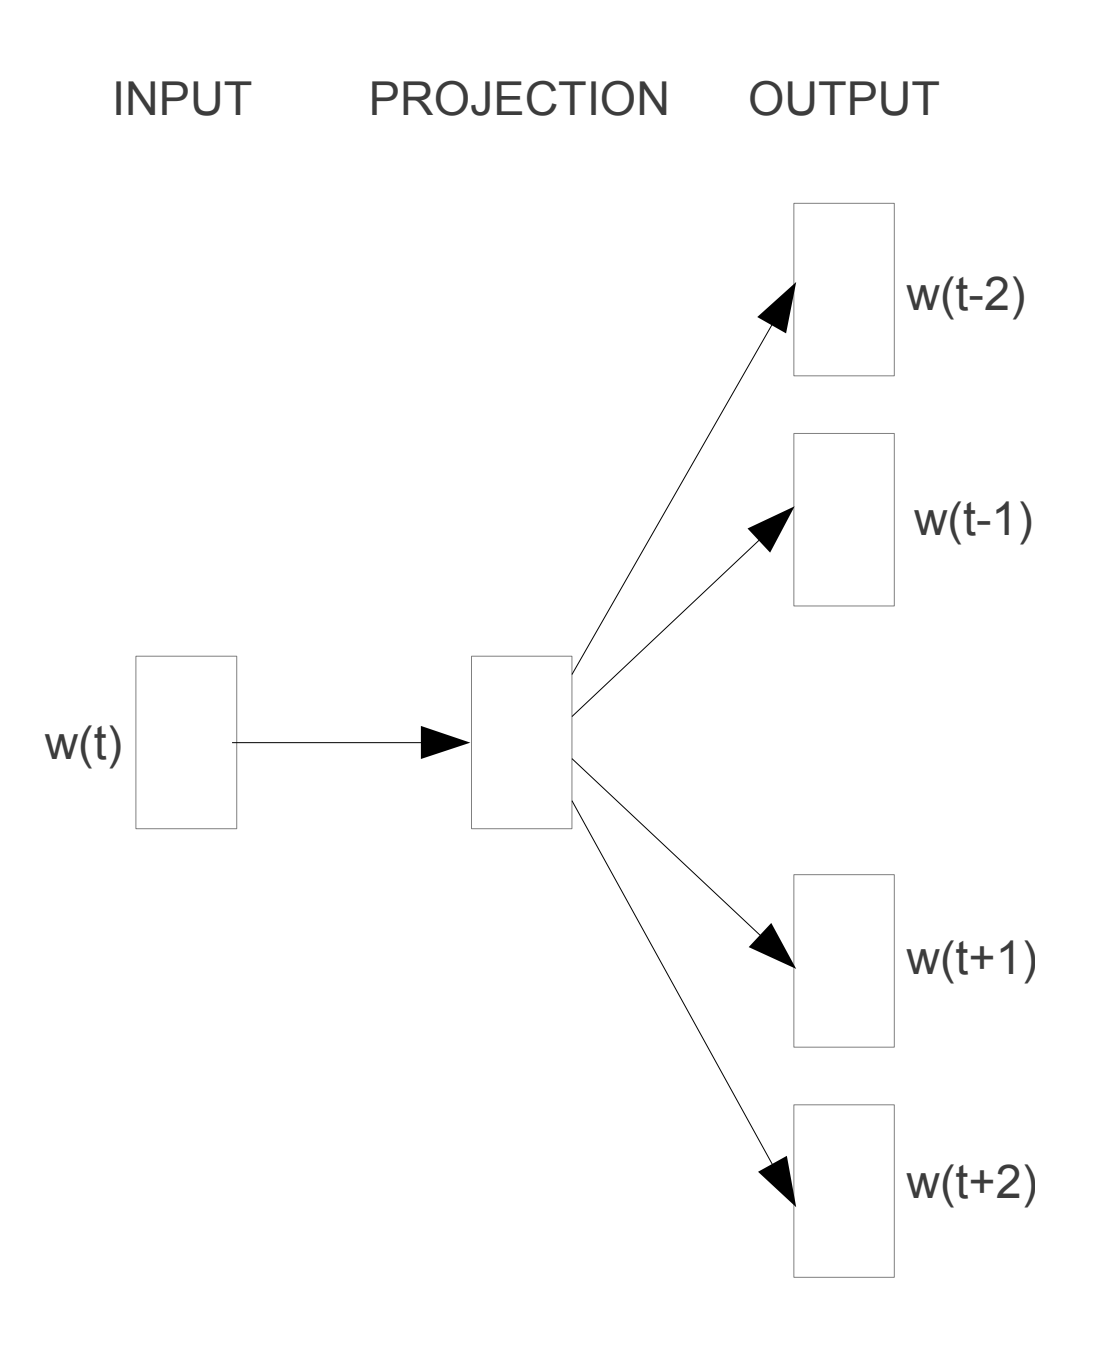
\includegraphics[width=8cm]{thesis/figures/skip-gram-mikolov-et-al-2013.png}
    \caption{The Skip-gram architecture as illustrated by Mikolov et al. \cite{mikolov2013a}}
    \label{fig:skip-gram-model}
\end{figure}

\noindent
As with the CBOW model, we have some target word $w_t$ with $C$ context words around it, $w_{t-C}, \ldots, w_{t-1}, w_{t+1}, \ldots, w_{t+C}$. The objective of the Skip-gram model \cite{mikolov2013b} then becomes
\begin{align}
    \frac{1}{T} \sumlim{t=1}{T} \sumlim{-C \leq j \leq C, j \neq 0}{} \log  p(w_{t+j} | w_t)
\end{align}

\noindent
Similar to CBOW, the Skip-gram model uses the two matrices $W$ and $W'$ for mapping from input to projection/hidden layer and projection/hidden layer to output respectively.

\noindent
Mikolov et al. reported that the Skip-gram model performed better than the CBOW model overall \cite{mikolov2013a}. For this reason and due to the scope of the masters thesis, we will stick to using the Skip-gram model throughout the thesis.

\subsection{Negative Sampling}

\noindent
In the Skip-gram model, we typically define $p(w_{t+j} | w_t)$ using the softmax function \cite{mikolov2013b} TODO: Reference softmax function?
\begin{align}
    p(w_{t+j} | w_t)
    &= \frac{\exp{ \left( \trans{v'_{t+j}} v_t \right) }} {\exp{  \sumlim{k=1}{|V|} \left( \trans{v'_k} v_t \right) }}
    \label{eqn:skip-gram-p-function}
\end{align}
where $v'_t$ and $v_t$ are the "input" and "output" vector representations of the word $w$, and $|V|$ is the number of words in the vocabulary. There are some downsides with this formulation, however. In practice, it becomes hard to compute since the summation in the denominator of equation \ref{eqn:skip-gram-p-function} depends on the number of words in the vocabulary, which is often large ($10^5 - 10^7$ terms) \cite{mikolov2013b}.

\noindent
To deal with the computational requirements of the original Skip-gram model, Mikolov et al. first showed how one might use hierarchical softmax \cite{mikolov2013b}. Hierarchical softmax is an efficient way of computing the softmax function; instead of evaluating $|V|$ words to compute the probability in equation \ref{eqn:skip-gram-p-function}, we only have to evaluate $\log \left( |V| \right)$ words \cite{mikolov2013b}.

\noindent
Following, Mikolov et al. introduce Negative sampling as an alternative to hierarchical softmax, which builds on the concept of distinguising a target word $w_t$ from a word randomly sampled from the vocabulary. In particular, we randomly sample words from the vocabulary using the unigram distribution raised to the power of $\alpha$ \cite{mikolov2013b}. The unigram distribution is a distribution for sampling a word at random from the vocabulary using the word occurrence counts, and the choice of raising it to the power of $\alpha = \frac{3}{4}$ was empirically found to be the best exponent. Furthermore, we will refer to this unigram distribution as the noise distribution $P_n(w)$ \cite{mikolov2013b}. Note that Negative sampling method can also be applied to CBOW in a similar manner \cite{mikolov2013b}.

\noindent
Before we can explain Negative sampling, we define the positive- and negative target-context pairs.
\begin{definition}
Given a vocabulary $V$, a target word $w_t$ and the target words contextual words $w_{t-C}, \ldots, w_{t-1}, w_{t+1}, \ldots, w_{t+C}$ for some window size $C$, we define a \textbf{positive target-context pair} to be the pair of the target word $w_t$ and a contextual word $w_{t+l}$, $-C \leq l \leq C, l \neq 0$, e.g., the pair $\left( w_t, w_{t+1} \right)$ for $l=1$. Furthermore, we define a \textbf{negative target-context pair} as the pair of the contextual word $w_{t+l}$ and a word $w_r$ randomly sampled from the noise distribution $P_n(w)$, e.g., the pair $\left( w_{t+l}, w_r \right)$.
\end{definition}

\noindent
In Negative sampling, we are only concerned with a subset of all the words in the vocabulary when computing the loss using the softmax function. For each word in the text we are training on, we create a positive target-context pair $\left( w_t, w_{t+l} \right)$, $-C \leq l \leq C, l \neq 0$. Furthermore, we generate $k$ negative target-context pairs for each word, where $k$ is in the range of $5-20$ for small training sets and $2-5$ for big training sets \cite{mikolov2013b}. We let $W_{np} = \left \{ w_j | j \in 1, \ldots, k \right \}$ be the set of $k$ negatively sampled words from the noise distribution $P_n(w)$. With these details in mind, the objective function of Negative sampling is \cite{mikolov2013b, rong2014word2vec}. TODO: Fix this equation, wronly stated at the moment.
\begin{align}
\log \sigma \left( \trans{w_t} w_{t+l} \right) + \sumlim{w_j \in W_{np}}{} \log \sigma \left( -\trans{w_j} w_{t+l} \right)
\label{eqn:negative-sampling-obj-func}
\end{align}
where $\sigma$ is the sigmoid function, e.g., $\sigma(z) = \frac{1}{1 + \exp{(-z)}}$. TODO: Reference sigmoid function?

\noindent
From equation \ref{eqn:negative-sampling-obj-func}, we see that we only have to compute for $(1 + k)$ words, which is a big improvement over computing for $|V|$ words (assuming that $|V|$ is much larger than $k$). Mikolov et al. also reports that by using Negative sampling, we increase the quality of the word embeddings \cite{mikolov2013b}.

\subsection{Subsampling of words}
When training a word2vec model, one usually has to train on big text corpora to achieve good quality of word embeddings \cite{mikolov2013a}. However, as the number of training words increase, the discrepancy between rare and frequent words increase as well. When using Negative sampling, we are sampling negative target-context pairs from the vocabulary, which depends on the unigram distribution. In English text corpora, words such as "the", "of", "is" can easily occur hundreds of millions of times and usually provide less information than more rare words \cite{mikolov2013b}. For this reason, we apply a simple, yet efficient subsampling scheme to counter the imbalance between rare and frequent words; before the text corpora is processed into target-context pairs, each word $w_t$ is discarded with the probability computed by the formula \cite{mikolov2013b, levy-etal-2015-improving}
\begin{equation}
    P_d(w_t) = 1 - \sqrt{\frac{t}{f(w_t)}}
\end{equation}
where $f(w_t)$ is the (relative) frequency of word $w_t$ and $t$ is a chosen threshold, usually around $10^{-5}$ \cite{mikolov2013b}.

\noindent
It should be noted, however, that in the source code of word2vec\footnote{\href{https://github.com/tmikolov/word2vec/blob/e092540633572b883e25b367938b0cca2cf3c0e7/word2vec.c\#L407}{word2vec.c at line 407 (of the original word2vec repository)}}, they use a slightly modified formula. We will use this formula when implementing word2vec.
\begin{align}
    P_d(w_t) = \frac{f(w_t) - t}{f(w_t)} - \sqrt{\frac{t}{f(w_t)}}
\end{align}

\subsection{Word2vec as an artificial neural network}
Typically in the literature, word2vec is presented using the equations \ref{eqn:cbow-objective-function}, \ref{eqn:skip-gram-p-function} and \ref{eqn:negative-sampling-obj-func}. We will, however, explain how to set word2vec up as an artificial neural network (ANN), in the sense that we will implement it later in the thesis. In particular, we will explain how to set up the Skip-gram model with negative sampling as an ANN. This ANN consists of three fully-connected layers of artificial neurons \cite{rong2014word2vec} and is illustrated in \figref{fig:word2vec-skip-gram-negative-sampling}.

\begin{figure}[ht]
    \centering
    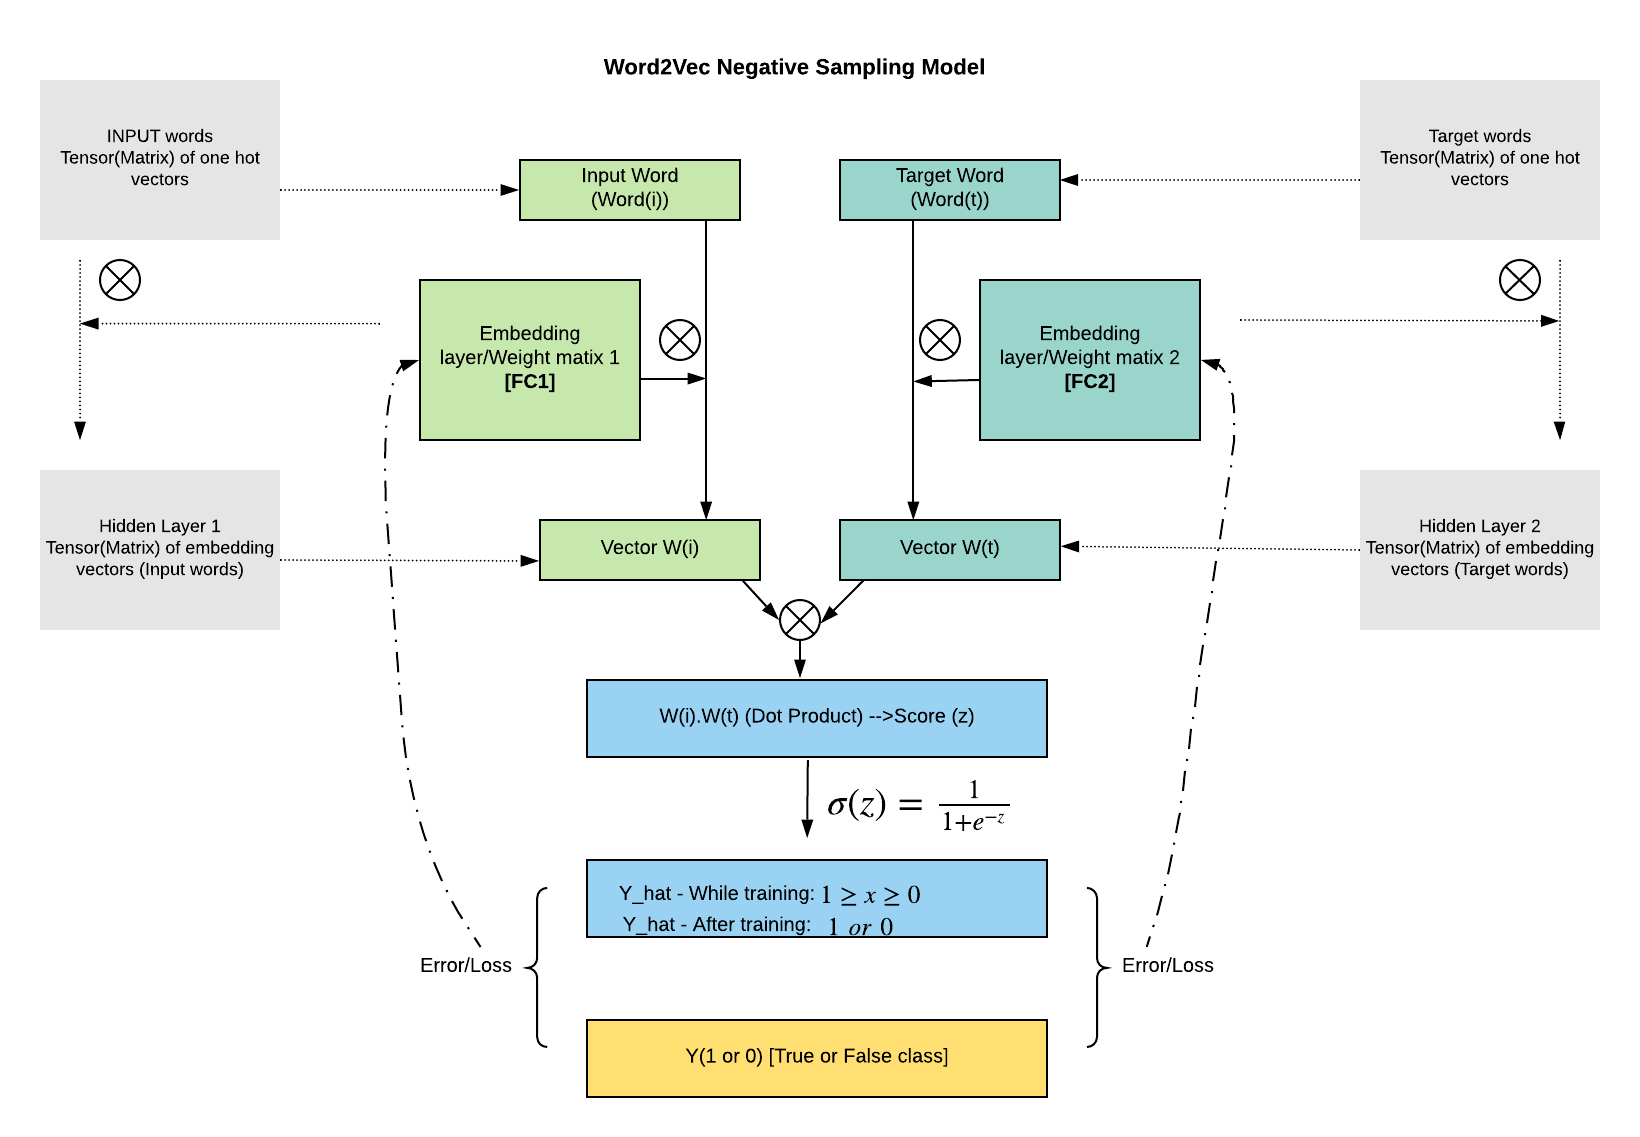
\includegraphics[width=12cm]{thesis/figures/word2vec-skip-gram-negative-sampling.png}
    \caption{TODO: Replace with TikZ illustration}
    \label{fig:word2vec-skip-gram-negative-sampling}
\end{figure}

\noindent
TODO: How to set it up, target vs context embedding, etc.

\section{Training a word2vec model}
TODO: Data preprocessing, Tensorflow, hyperparameters, etc.

\section{Evaluating a word2vec model}
TODO: Semantic and syntactic relations
\chapter{Analysis of Embeddings}
TODO

\section{Cluster analysis}
TODO

\subsection{Comparing clustering algorithms}
TODO

\subsection{Clustering word groups}
TODO
\chapter{Topological Analysis}
TODO
\section{Conclusion}
\label{sec:conclusion}
To conclude the thesis, we obtain meaningful clusters of word embeddings when we apply them to clustering algorithms and validate the result using internal cluster validation methods. Additionally, topological polysemy does not seem to measure the polysemy of words efficiently and consistently. We note that the topological polysemy method is a relatively new idea, and it requires more work to find out more about the algorithm and its results. In the next chapter, we will discuss our ideas for future work related to this thesis.

% Include more chapters as required.
%%=========================================
\renewcommand{\glossarypreamble}{\footnotesize}
\printglossary[style=super, type=\glsdefaulttype] \let\cleardoublepage\clearpage
\printglossary[style=super, type=\acronymtype]
% Include more appendices as required.
%%=========================================
\clearpage
\DeclareRobustCommand{\VAN}[3]{#3}
\addcontentsline{toc}{chapter}{Bibliography}
\bibliographystyle{apalike}
\bibliography{generators/refs}
\appendix
\titleformat{\chapter}[display]
  {\normalfont\large\bfseries}% <- font for label "Appendix A", default \huge
  {\chaptertitlename\ \thechapter}
  {20pt}
  {\large}% <- font for title, default \Huge

\chapter{Generated code from Protocol buffers}

\begin{lstlisting}[caption={Source code of something},label=Listing]
System.out.println("Hello Mars");
\end{lstlisting}
\end{document}